\documentclass{vkr}
\usepackage[english, russian]{babel} % переносы
\usepackage{graphicx} % для вставки картинок
\graphicspath{{images/}} % путь к изображениям
\usepackage[hidelinks]{hyperref}
\usepackage{float} % определяет метод H для рисунка с переносом на следующую страницу, ели не помещается
\usepackage{pdflscape}
\addto{\captionsrussian}{\renewcommand{\refname}{СПИСОК ИСПОЛЬЗОВАННЫХ ИСТОЧНИКОВ}}
\usepackage{xltabular} % для вставки таблиц
\usepackage{makecell}
\renewcommand\theadfont{} % шрифт в /thead
\usepackage{array} % для определения новых типов столбцов таблиц
\newcolumntype{T}{>{\centering\arraybackslash}X} % новый тип столбца T - автоматическая ширина столбца с выравниванием по центру
\newcolumntype{R}{>{\raggedleft\arraybackslash}X} % новый тип столбца R - автоматическая ширина столбца с выравниванием по правому краю
\newcolumntype{C}[1]{>{\centering\let\newline\\\arraybackslash\hspace{0pt}}m{#1}} % новый тип столбца C - фиксированная ширина столбца с выравниванием по центру
\newcolumntype{r}[1]{>{\raggedleft\arraybackslash}p{#1}} % новый тип столбца r - фиксированная ширина столбца с выравниванием по правому краю
\newcommand{\centrow}{\centering\arraybackslash} % командой \centrow можно центрировать одну ячейку (заголовок) в столбце типа X или p, оставив в оcтальных ячейках другой тип выравнивания
\newcommand{\finishhead}{\endhead\hline\endlastfoot}
\newcommand{\continuecaption}[1]{\captionsetup{labelformat=empty} \caption[]{#1}\\ \hline }
\usepackage{etoolbox}
\AtBeginEnvironment{xltabular}{\refstepcounter{tablecnt}} % подсчет таблиц xltabular, обычные таблицы подсчитываются в классе

\usepackage[tableposition=top]{caption} % подпись таблицы вверху
\captionsetup{strut=off}
\setlength{\intextsep}{0pt} % Vertical space above & below [h] floats
\setlength{\textfloatsep}{0pt} % Vertical space below (above) [t] ([b]) floats
\DeclareCaptionLabelFormat{gostfigure}{Рисунок #2} %подпись рисунка
\DeclareCaptionLabelFormat{gosttable}{Таблица #2} %подпись таблицы
\DeclareCaptionLabelSeparator{gost}{~--~} %разделитель в рисунках и таблицах
\captionsetup{labelsep=gost}
\captionsetup[figure]{aboveskip=10pt,belowskip=4mm,justification=centering,labelformat=gostfigure} % настройка подписи рисунка
\captionsetup[table]{font={stretch=1.41},skip=0pt,belowskip=0pt,aboveskip=8.5pt,singlelinecheck=off,labelformat=gosttable} % настройка подписи таблицы

\setlength{\LTpre}{8mm} % отступ сверху таблицы
\setlength{\LTpost}{6mm} % отступ снизу таблицы

\usepackage{enumitem}
\setlist{nolistsep,wide=\parindent,itemindent=*} % отступы вокруг списков, выравнивание с учетом разделителя

\usepackage{color} %% это для отображения цвета в коде
\usepackage{listings} %% листинги кода
\setmonofont[Scale=0.7]{Verdana} % моноширный шрифт для листинга

\definecolor{codegreen}{rgb}{0,0.6,0}
\definecolor{codegray}{rgb}{0.5,0.5,0.5}
\definecolor{codepurple}{rgb}{0.58,0,0.82}

\lstset{ %
language=C,                 % выбор языка для подсветки (здесь это С)
numbers=left,               % где поставить нумерацию строк (слева\справа)
numberstyle=\tiny,           % размер шрифта для номеров строк
stepnumber=1,                   % размер шага между двумя номерами строк
numbersep=5pt,                % как далеко отстоят номера строк от подсвечиваемого кода
commentstyle=\color{codegreen},
keywordstyle=\color{magenta},
numberstyle=\tiny\color{codegray},
stringstyle=\color{codepurple},
basicstyle=\linespread{0.95}\ttfamily,
backgroundcolor=\color{white}, % цвет фона подсветки - используем \usepackage{color}
showspaces=false,            % показывать или нет пробелы специальными отступами
showstringspaces=false,      % показывать или нет пробелы в строках
showtabs=false,             % показывать или нет табуляцию в строках
frame=single,              % рисовать рамку вокруг кода
tabsize=2,                 % размер табуляции по умолчанию равен 2 пробелам
captionpos=t,              % позиция заголовка вверху [t] или внизу [b] 
breaklines=true,           % автоматически переносить строки (да\нет)
breakatwhitespace=false, % переносить строки только если есть пробел
escapeinside={\%*}{*)}   % если нужно добавить комментарии в коде
}

\makeatletter % чтобы допускались русские комментарии в листингах
\lst@InputCatcodes
\def\lst@DefEC{%
 \lst@CCECUse \lst@ProcessLetter
  ^^80^^81^^82^^83^^84^^85^^86^^87^^88^^89^^8a^^8b^^8c^^8d^^8e^^8f%
  ^^90^^91^^92^^93^^94^^95^^96^^97^^98^^99^^9a^^9b^^9c^^9d^^9e^^9f%
  ^^a0^^a1^^a2^^a3^^a4^^a5^^a6^^a7^^a8^^a9^^aa^^ab^^ac^^ad^^ae^^af%
  ^^b0^^b1^^b2^^b3^^b4^^b5^^b6^^b7^^b8^^b9^^ba^^bb^^bc^^bd^^be^^bf%
  ^^c0^^c1^^c2^^c3^^c4^^c5^^c6^^c7^^c8^^c9^^ca^^cb^^cc^^cd^^ce^^cf%
  ^^d0^^d1^^d2^^d3^^d4^^d5^^d6^^d7^^d8^^d9^^da^^db^^dc^^dd^^de^^df%
  ^^e0^^e1^^e2^^e3^^e4^^e5^^e6^^e7^^e8^^e9^^ea^^eb^^ec^^ed^^ee^^ef%
  ^^f0^^f1^^f2^^f3^^f4^^f5^^f6^^f7^^f8^^f9^^fa^^fb^^fc^^fd^^fe^^ff%
  ^^^^20ac^^^^0153^^^^0152%
  % Basic Cyrillic alphabet coverage
  ^^^^0410^^^^0411^^^^0412^^^^0413^^^^0414^^^^0415^^^^0416^^^^0417%
  ^^^^0418^^^^0419^^^^041a^^^^041b^^^^041c^^^^041d^^^^041e^^^^041f%
  ^^^^0420^^^^0421^^^^0422^^^^0423^^^^0424^^^^0425^^^^0426^^^^0427%
  ^^^^0428^^^^0429^^^^042a^^^^042b^^^^042c^^^^042d^^^^042e^^^^042f%
  ^^^^0430^^^^0431^^^^0432^^^^0433^^^^0434^^^^0435^^^^0436^^^^0437%
  ^^^^0438^^^^0439^^^^043a^^^^043b^^^^043c^^^^043d^^^^043e^^^^043f%
  ^^^^0440^^^^0441^^^^0442^^^^0443^^^^0444^^^^0445^^^^0446^^^^0447%
  ^^^^0448^^^^0449^^^^044a^^^^044b^^^^044c^^^^044d^^^^044e^^^^044f%
  ^^^^0401^^^^0451%
  %%%
  ^^00}
\lst@RestoreCatcodes
\makeatother


% Режим шаблона (должен быть включен один из трех)
\ВКРtrue
%\Практикаtrue
%\Курсоваяtrue

\newcommand{\Дисциплина}{<<Проектирование и архитектура программных систем>>} % для курсовой
\newcommand{\КодСпециальности}{09.03.04} % Курсовая
\newcommand{\Специальность}{Программная инженерия} % Курсовая
\newcommand{\Тема}{Маркетплейс для реализации цифровых предметов внутри игры «Stay Out»} % ВКР Курсовая
\newcommand{\ТемаВтораяСтрока}{}
\newcommand{\ГдеПроводитсяПрактика}{ООО "Предприятие ВТИ-Сервис"} % для практики
\newcommand{\РуководительПрактПредпр}{Федосов Д. В.} % для практики
\newcommand{\ДолжнРуководительПрактПредпр}{директор} % для практики
\newcommand{\РуководительПрактУнивер}{Чаплыгин А. А.} % для практики
\newcommand{\ДолжнРуководительПрактУнивер}{к.т.н. доцент} % для практики
\newcommand{\Автор}{В. Е. Зеленцов}
\newcommand{\АвторРод}{Зеленцова В. Е.}
\newcommand{\АвторПолностьюРод}{Зеленцова Виталия Евгеньевича} % для практики
\newcommand{\Шифр}{20-06-0045}
\newcommand{\Курс}{4} % для практики
\newcommand{\Группа}{ПО-01б}
\newcommand{\Руководитель}{В. В. Серебровский} % для ВКР и курсовой
\newcommand{\Нормоконтроль}{А. А. Чаплыгин} % для ВКР
\newcommand{\ЗавКаф}{А. В. Малышев} % для ВКР
\newcommand{\ДатаПриказа}{«04» апреля 2024~г.} % для ВКР
\newcommand{\НомерПриказа}{1616-с} % для ВКР
\newcommand{\СрокПредоставления}{«11» июня 2024~г.} % для ВКР, курсового

\begin{document}
\maketitle
\ifПрактика{}\else{
   \newpage
\begin{center}
\large\textbf{Минобрнауки России}

\large\textbf{Юго-Западный государственный университет}
\vskip 1em
\normalsize{Кафедра программной инженерии}
\vskip 1em
\ifВКР{
        \begin{flushright}
        \begin{tabular}{p{.4\textwidth}}
        \centrow УТВЕРЖДАЮ: \\
        \centrow Заведующий кафедрой \\
        \hrulefill \\
        \setarstrut{\footnotesize}
        \centrow\footnotesize{(подпись, инициалы, фамилия)}\\
        \restorearstrut
        «\underline{\hspace{1cm}}»
        \underline{\hspace{3cm}}
        20\underline{\hspace{1cm}} г.\\
        \end{tabular}
        \end{flushright}
        }\fi
\end{center}
\vspace{1em}
  \begin{center}
  \large
\ifВКР{
ЗАДАНИЕ НА ВЫПУСКНУЮ КВАЛИФИКАЦИОННУЮ РАБОТУ
  ПО ПРОГРАММЕ БАКАЛАВРИАТА}
  \else
ЗАДАНИЕ НА КУРСОВУЮ РАБОТУ (ПРОЕКТ)
\fi
\normalsize
  \end{center}
\vspace{1em}
{\parindent0pt
  Студента \АвторРод, шифр\ \Шифр, группа \Группа
  
1. Тема «\Тема\ \ТемаВтораяСтрока»
\ifВКР{
утверждена приказом ректора ЮЗГУ от \ДатаПриказа\ № \НомерПриказа
}\fi.

2. Срок предоставления работы к защите \СрокПредоставления

3. Исходные данные для создания программной системы:

3.1. Перечень решаемых задач:}

\renewcommand\labelenumi{\theenumi)}

\begin{enumerate}
\item Провести анализ предметной области;
\item Разработать концептуальную модель программной системы;
\item Спроектировать и реализовать серверную часть программной системы;
\item Спроектировать и реализовать клиентскую часть программной системы;
\item Провести тестирование работы программной системы.
\end{enumerate}

{\parindent0pt
  3.2. Входные данные и требуемые результаты для программы:}

\begin{enumerate}
\item Входными данными для программной системы являются: параметры фильтрации ленты товаров; данные для авторизации и регистрации пользователя; сведения о товарах.
\item Выходными данными для программной системы являются: отфильтрованные и отсортированные списки товаров;пуш-уведомления с информацией о событиях; уникальные токены для автоматической авторизации.
\end{enumerate}

{\parindent0pt

  4. Содержание работы (по разделам):
  
  4.1. Введение
  
  4.1. Анализ предметной области
  
4.2. Техническое задание: основание для разработки, назначение разработки,
требования к программной системе, требования к оформлению документации.

4.3. Технический проект: общие сведения о программной системе, проект
данных программной системы, проектирование архитектуры программной системы, проектирование пользовательского интерфейса программной системы.

4.4. Рабочий проект: спецификация компонентов и классов программной системы, тестирование программной системы, сборка компонентов программной системы.

4.5. Заключение

4.6. Список использованных источников

5. Перечень графического материала:

\списокПлакатов

\vskip 2em
\begin{tabular}{p{6.8cm}C{3.8cm}C{4.8cm}}
Руководитель \ifВКР{ВКР}\else работы (проекта) \fi & \lhrulefill{\fill} & \fillcenter\Руководитель\\
\setarstrut{\footnotesize}
& \footnotesize{(подпись, дата)} & \footnotesize{(инициалы, фамилия)}\\
\restorearstrut
Задание принял к исполнению & \lhrulefill{\fill} & \fillcenter\Автор\\
\setarstrut{\footnotesize}
& \footnotesize{(подпись, дата)} & \footnotesize{(инициалы, фамилия)}\\
\restorearstrut
\end{tabular}
}

\renewcommand\labelenumi{\theenumi.}

   \abstract{РЕФЕРАТ}

Объем работы равен \formbytotal{lastpage}{страниц}{е}{ам}{ам}. Работа содержит \formbytotal{figurecnt}{иллюстраци}{ю}{и}{й}, \formbytotal{tablecnt}{таблиц}{у}{ы}{}, \arabic{bibcount} библиографических источников и \formbytotal{числоПлакатов}{лист}{}{а}{ов} графического материала. Количество приложений – 2. Графический материал представлен в приложении А. Фрагменты исходного кода представлены в приложении Б.

Перечень ключевых слов: внутриигровые ценности, онлайн-торговая площадка, маркетплейс, Stay Out, React, Express, услуги, сервисы, разработка, информационные технологии, аутентификация, классы, база данных, средства защиты информации, компонент, модуль, сущность, информационный блок, метод, администратор, пользователь, web-сайт, диаграмма

Объектом разработки является маркетплейс для реализации внутриигровых ценностей в игре Stay Out.

Целью выпускной квалификационной работы является разработка и реализация маркетплейса для внутриигровой торговли, обеспечивающего более доступный и дешевый способ обмена ценностями, а также надежность и простоту в использовании.

В процессе разработки маркетплейса были выделены основные сущности путем создания информационных блоков, разработаны классы и методы модулей, обеспечивающие работу с сущностями предметной области, а также корректную работу web-сайта, разработаны страницы, содержащие информацию о пользователе и предметах, выставленных на продажу, разработаны модули для добавления и удаления товаров.

\selectlanguage{english}
\abstract{ABSTRACT}
  
The volume of work is \formbytotal{lastpage}{page}{}{s}{s}. The work contains \formbytotal{figurecnt}{illustration}{}{s}{s}, \formbytotal{tablecnt}{table}{}{s}{s}, \arabic{bibcount} bibliographic sources and \formbytotal{числоПлакатов}{sheet}{}{s}{s} of graphic material. The number of applications is 2. The graphic material is presented in annex A. The layout of the site, including the connection of components, is presented in annex B.

List of keywords: in-game values, online trading platform, marketplace, Stay Out, React, Express, services, services, development, information technology, authentication, classes, database, information security tools, component, module, entity, information block, method, administrator, user, website, diagram

The object of development is a marketplace for the implementation of in-game values ​​in the Stay Out game.

The goal of the final qualifying work is to develop and implement a marketplace for in-game trading, providing a more accessible and cheaper way to exchange values, as well as reliability and ease of use.

In the process of developing the marketplace, the main entities were identified by creating information blocks, module classes and methods were developed to ensure work with domain entities, as well as the correct operation of the website, pages containing information about the user and items for sale were developed, modules were developed to add and remove products.
\selectlanguage{russian}
}\fi
\tableofcontents
\section*{ОБОЗНАЧЕНИЯ И СОКРАЩЕНИЯ}

БД -- база данных.
ИС -- информационная система.
ИТ -- информационные технологии. 
ПО -- программное обеспечение.
РП -- рабочий проект.
СУБД -- система управления базами данных.
ТЗ -- техническое задание.
ТП -- технический проект.
API (Application Programming Interface) -- набор определений и протоколов, которые позволяют различным программным приложениям взаимодействовать друг с другом.
UML (Unified Modelling Language) -- язык графического описания для объектного моделирования в области разработки программного обеспечения.
MMORPG (massively multiplayer online role-playing game) -- компьютерная игра, в которой жанр ролевых игр совмещается с жанром массовых онлайн-игр.

\ifПрактика{}\else{\section*{ВВЕДЕНИЕ}
\addcontentsline{toc}{section}{ВВЕДЕНИЕ}

В мире массовых многопользовательских онлайн-игр жанра MMORPG, таких, как «Stay Out», игроки могут взаимодействовать в виртуальном мире, выполнять квесты, сражаться с монстрами, развивать своих персонажей и, конечно же, торговать внутри игровыми ценностями. MMORPG представляют собой уникальный игровой жанр, где тысячи игроков со всего мира могут взаимодействовать между собой в одном виртуальном мире, создавая атмосферу постоянного развития и приключений.

Сервис для обмена и продажи виртуальных ценностей в MMORPG
призван упростить процесс торговли между игроками, предоставляя им удобную платформу для взаимодействия. Необходимость в таком сервисе возникает из-за того, что в некоторых играх обмен виртуальными ценностями может быть неудобным и невыгодным для игроков. Это может приводить к созданию различных групп в социальных сетях и мессенджерах, где игроки
выкладывают свои товары и договариваются о сделках.

Целью таких сервисов является упрощение процесса торговли, делая
его более удобным и безопасным для всех участников. Путем создания специализированной платформы для обмена и продажи виртуальных ценностей, игрокам будет легче находить нужные товары, договариваться о цене и завершать сделки, минимизируя риск обмана и недобросовестных сделок.

Преимущества сервиса для обмена виртуальными ценностями:
\begin{itemize}
	\item сервис не требует значительных ресурсов для использования и позволяет игрокам свободно обмениваться своими предметами;
	\item пользователи могут легко связываться друг с другом, договариваться о цене и условиях сделки, что делает процесс торговли более удобным и эффективным;
	\item  в сервисах для обмена виртуальными ценностями нет лишней административной информации и правил, устанавливаемых владельцем группы или сообщества, что делает процесс торговли более прозрачным и справедливым для всех участников.
\end{itemize}

\emph{Цель настоящей работы} – разработка web-сайта для упрощения торговли в игре «Stay Out», ввиду отсутствия каких-либо хороших альтернатив. Для достижения поставленной цели необходимо решить \emph{следующие задачи:}
\begin{itemize}
	\item провести анализ предметной области;
	\item разработать концептуальную модель программной системы;
	\item спроектировать и реализовать серверную часть программной системы;
	\item спроектировать и реализовать клиентскую часть программной системы;
	\item провести тестирование работы программной системы.
\end{itemize}

\emph{Структура и объем работы.} Отчет состоит из введения, 4 разделов основной части, заключения, списка использованных источников, 2 приложений. Текст выпускной квалификационной работы равен \formbytotal{lastpage}{страниц}{е}{ам}{ам}.

\emph{Во введении} сформулирована цель работы, поставлены задачи разработки, описана структура работы, приведено краткое содержание каждого из разделов.

\emph{В первом разделе} на стадии описания технической характеристики предметной области приводится сбор информации о деятельности компании, для которой осуществляется разработка сайта.

\emph{Во втором разделе} на стадии технического задания приводятся требования к разрабатываемому сайту.

\emph{В третьем разделе} на стадии технического проектирования представлены проектные решения для web-сайта.

\emph{В четвертом разделе} приводится список классов и их методов, использованных при разработке сайта, производится тестирование разработанного сайта.

В заключении излагаются основные результаты работы, полученные в ходе разработки.

В приложении А представлен графический материал.
В приложении Б представлены фрагменты исходного кода. 
}\fi
\section{Анализ предметной области}
\subsection{Понятия и принципы маркетплейса}

\subsubsection{Определение маркетплейса}
Маркетплейс -- платформа электронной коммерции, интернет-магазин электронной торговли, предоставляющий информацию о продукте или услуге третьих лиц. Его особенность в том, что один и тот же товар зачастую можно купить у нескольких продавцов, при этом цена на товар может различаться. В пример успешных маркетплейсов можно привести Aliexpress и Wildberries.

\paragraph{Aliexpress}
Aliexpress — это один из крупнейших мировых маркетплейсов, принадлежащий китайской компании Alibaba Group. Платформа была запущена в 2010 году и с тех пор значительно расширила свою деятельность, предлагая товары от множества китайских производителей и продавцов. Aliexpress предоставляет покупателям возможность приобретать широкий ассортимент товаров, начиная от электроники и заканчивая одеждой и аксессуарами, часто по конкурентоспособным ценам. Благодаря удобной системе отзывов и рейтингов, покупатели могут легко оценить качество товаров и уровень обслуживания продавцов.

\paragraph{Wildberries}
Wildberries — один из крупнейших российских маркетплейсов, который был основан в 2004 году. Платформа предлагает широкий ассортимент товаров, включая одежду, обувь, электронику, товары для дома и многое другое. Wildberries отличается быстрой доставкой и широкой сетью пунктов выдачи заказов по всей России. Платформа также активно развивает свою логистическую инфраструктуру, что позволяет эффективно обслуживать покупателей и обеспечивать высокое качество доставки.

\subsubsection{Принципы работы маркетплейсов}
Основные принципы работы маркетплейсов включают в себя:
\begin{itemize}
	\item \textbf{Платформа как посредник:} Маркетплейс выступает в роли посредника между покупателями и продавцами, предоставляя им удобный интерфейс для взаимодействия и проведения транзакций.
	\item \textbf{Механизмы доверия:} Для обеспечения доверия между участниками рынка маркетплейсы внедряют системы отзывов и рейтингов, которые помогают покупателям делать осознанный выбор, а продавцам улучшать качество своих товаров и услуг.
	\item \textbf{Поддержка транзакций:} Маркетплейсы обеспечивают безопасные методы оплаты и защиты данных, что способствует увеличению доверия и безопасности сделок.
\end{itemize}

\subsubsection{Разновидности маркетплейсов}
Существует несколько основных типов маркетплейсов в зависимости от характера взаимодействия между участниками:
\begin{itemize}
	\item \textbf{B2B (бизнес-бизнес):} Маркетплейсы, которые связывают между собой бизнесы. Интернет-платформы позволяют упростить торговлю на всех этапах, что в свою очередь открывает возможность сделать ее более оперативной и прозрачной.
	\item \textbf{B2C (бизнес-потребитель):} Маркетплейсы, где бизнесы продают товары непосредственно конечным потребителям. Очень схож по смыслу с B2B, но с тем различием, что продажа товаров должна осуществляться конечным пользователям.
	\item \textbf{C2C (потребитель-поребитель):} Маркетплейсы, где пользователи могут продавать товары друг другу. Данная схема приобретает все большую популярность в наше время. Она удобна тем, что товары обычно имеют более низкую стоимость, по сравнению со стоимостью в магазинах.
\end{itemize}

\subsection{Роль маркетплейсов в современной цифровой экономике}

Маркетплейсы играют значительную роль в современной цифровой экономике, изменяя способы взаимодействия между продавцами и покупателями, стимулируя конкуренцию и инновации, создавая новые рынки и улучшая потребительский опыт. В этом разделе мы рассмотрим основные аспекты, подчеркивающие важность маркетплейсов в современном экономическом ландшафте.

\subsubsection{Облегчение доступа к товарам и услугам}
Одним из ключевых преимуществ маркетплейсов является их способность предоставлять покупателям удобный доступ к широкому ассортименту товаров и услуг. Маркетплейсы функционируют как централизованные платформы, где можно найти товары различных категорий от множества продавцов. Это значительно упрощает процесс поиска и покупки нужных товаров, поскольку пользователи могут осуществлять все свои покупки в одном месте, вместо того чтобы искать различные товары на разных сайтах.

Кроме того, маркетплейсы работают круглосуточно, предоставляя покупателям возможность совершать покупки в любое удобное для них время. Это особенно важно в условиях глобализации, когда покупатели могут находиться в разных часовых поясах и иметь разные графики работы.

Примером такого подхода является Aliexpress, который предоставляет доступ к миллионам товаров от китайских производителей покупателям со всего мира. Доступность товаров и удобство совершения покупок делают маркетплейсы привлекательными как для потребителей, так и для продавцов.

\subsubsection{Стимулирование конкуренции и инноваций}
Маркетплейсы способствуют усилению конкуренции среди продавцов, что в свою очередь стимулирует инновации и улучшение качества товаров и услуг. На маркетплейсах продавцы конкурируют не только ценой, но и качеством товаров, уровнем обслуживания и условиями доставки. Это создает благоприятные условия для появления инновационных решений и улучшений, направленных на удовлетворение потребностей покупателей.

Системы отзывов и рейтингов, внедренные на многих маркетплейсах, помогают покупателям принимать обоснованные решения о покупке и повышают уровень доверия к продавцам. Продавцы, стремящиеся к высоким рейтингам и положительным отзывам, вынуждены улучшать свои товары и сервисы, что в конечном итоге выгодно потребителям.

Маркетплейсы также являются платформами для внедрения новых технологий, таких как искусственный интеллект, анализ данных и персонализация. Эти технологии помогают улучшать пользовательский опыт, предлагать более точные рекомендации и оптимизировать процессы логистики и доставки.

\subsubsection{Создание новых рынков и возможностей для предпринимателей}
Маркетплейсы предоставляют малым и средним предприятиям (МСП) уникальные возможности для выхода на рынок и расширения своей клиентской базы. Благодаря маркетплейсам МСП могут получить доступ к глобальной аудитории, не затрачивая значительные ресурсы на создание и продвижение собственного интернет-магазина.

Платформы маркетплейсов предлагают предпринимателям готовую инфраструктуру для продажи товаров, включая системы оплаты, логистики и маркетинга. Это позволяет предприятиям сосредоточиться на производстве и улучшении товаров, оставляя технические и организационные вопросы на платформу.

Российский маркетплейс Wildberries является примером успешной интеграции малого и среднего бизнеса в онлайн-торговлю. Платформа предоставляет продавцам доступ к широкой аудитории и помогает им на всех этапах продаж, от регистрации и размещения товаров до логистики и обслуживания клиентов.

\subsubsection{Улучшение потребительского опыта}
Маркетплейсы значительно улучшают потребительский опыт за счет персонализированных рекомендаций, удобных интерфейсов и разнообразия вариантов доставки. Платформы используют данные о поведении пользователей для предложения товаров, которые наиболее соответствуют их предпочтениям и потребностям. Это не только повышает удовлетворенность клиентов, но и увеличивает вероятность повторных покупок.

Удобные интерфейсы и простота навигации делают процесс покупки быстрым и приятным. Покупатели могут легко сравнивать товары, читать отзывы других пользователей и принимать обоснованные решения о покупке. Возможность выбора из различных вариантов доставки, включая экспресс-доставку и самовывоз, также повышает удобство и удовлетворенность покупателей.

Маркетплейсы активно развивают свои логистические сети, что позволяет им предлагать быструю и надежную доставку. Например, Wildberries инвестирует в создание собственных складов и пунктов выдачи заказов по всей России, что значительно ускоряет процесс доставки и улучшает качество обслуживания клиентов.

В заключение, маркетплейсы играют ключевую роль в современной цифровой экономике, предоставляя покупателям удобный доступ к товарам и услугам, стимулируя конкуренцию и инновации, создавая новые рынки для предпринимателей и улучшая потребительский опыт. Их влияние на экономику продолжает расти, предлагая новые возможности для бизнеса и улучшая качество жизни потребителей.





\section{Техническое задание}
\subsection{Основание для разработки}

Полное наименование системы: "<Маркетплейс для реализации цифровых предметов внутри игры «Stay Out»">.

Основанием для разработки программы является приказ ректора ЮЗГУ от «07» апреля 2023 г. №1620-с «Об утверждении тем выпускных квалификационных работ».

\subsection{Цель и назначение разработки}

Основное назначение разработки маркетплейса для реализации цифровых предметов внутри игры «Stay Out» заключается в создании интегрированной платформы, которая обеспечит удобный и безопасный способ обмена, покупки и продажи внутриигровых предметов. Маркетплейс призван решать несколько ключевых задач:

\subsubsection{Удовлетворение потребностей игроков}
Маркетплейс предоставляет игрокам возможность легко покупать, продавать и обменивать цифровые предметы, такие как оружие, скины, внутриигровая валюта и другие уникальные объекты. Это позволяет игрокам разнообразить игровой процесс, улучшать свои игровые персонажи и получать больше удовольствия от игры.

\subsubsection{Увеличение вовлеченности и удержания игроков}
Интеграция маркетплейса стимулирует игроков проводить больше времени в игре, так как они получают дополнительные возможности для взаимодействия и торговли. Это способствует увеличению вовлеченности и удержания игроков, что в конечном итоге повышает популярность и доходность игры.

\subsubsection{Создание устойчивой игровой экономики}
Маркетплейс способствует формированию устойчивой игровой экономики, где игроки могут зарабатывать внутриигровую валюту и ресурсы, продавая свои предметы другим игрокам. Это создает динамичную и самоподдерживающуюся экосистему, которая улучшает общий игровой опыт и делает игру более интересной и реалистичной.

\subsubsection{Обеспечение безопасности транзакций}
Одной из ключевых задач разработки маркетплейса является обеспечение безопасности всех транзакций. Это включает в себя защиту данных пользователей, предотвращение мошенничества и обеспечение прозрачности всех операций. Надежные механизмы безопасности повышают доверие игроков к платформе и делают процесс торговли безопасным и надежным.

\subsubsection{Создание новых источников дохода для разработчиков}
Маркетплейс открывает новые возможности для монетизации игры, предоставляя разработчикам дополнительные источники дохода. Это может включать комиссионные с продаж, платные подписки для доступа к эксклюзивным предметам и другие модели дохода. Таким образом, маркетплейс помогает разработчикам инвестировать в дальнейшее развитие и улучшение игры.

\subsubsection{Улучшение взаимодействия внутри игрового сообщества}
Маркетплейс способствует улучшению взаимодействия между игроками, создавая платформу для обмена и торговли. Это помогает формировать более тесное и активное сообщество, где игроки могут делиться своими достижениями и получать поддержку от других участников.

В заключение, разработка маркетплейса для игры «Stay Out» направлена на создание удобного, безопасного и функционального инструмента для торговли цифровыми предметами, который будет способствовать развитию игровой экономики, увеличению вовлеченности игроков и созданию новых возможностей для монетизации игры.


\subsection{Требованияк программной системе}

\subsubsection{Требования к данным программной системы}

Концептуальная модель данных программной системы представлена на рисунке ~\ref{fig:modelbd}.

\begin{figure}[h]
	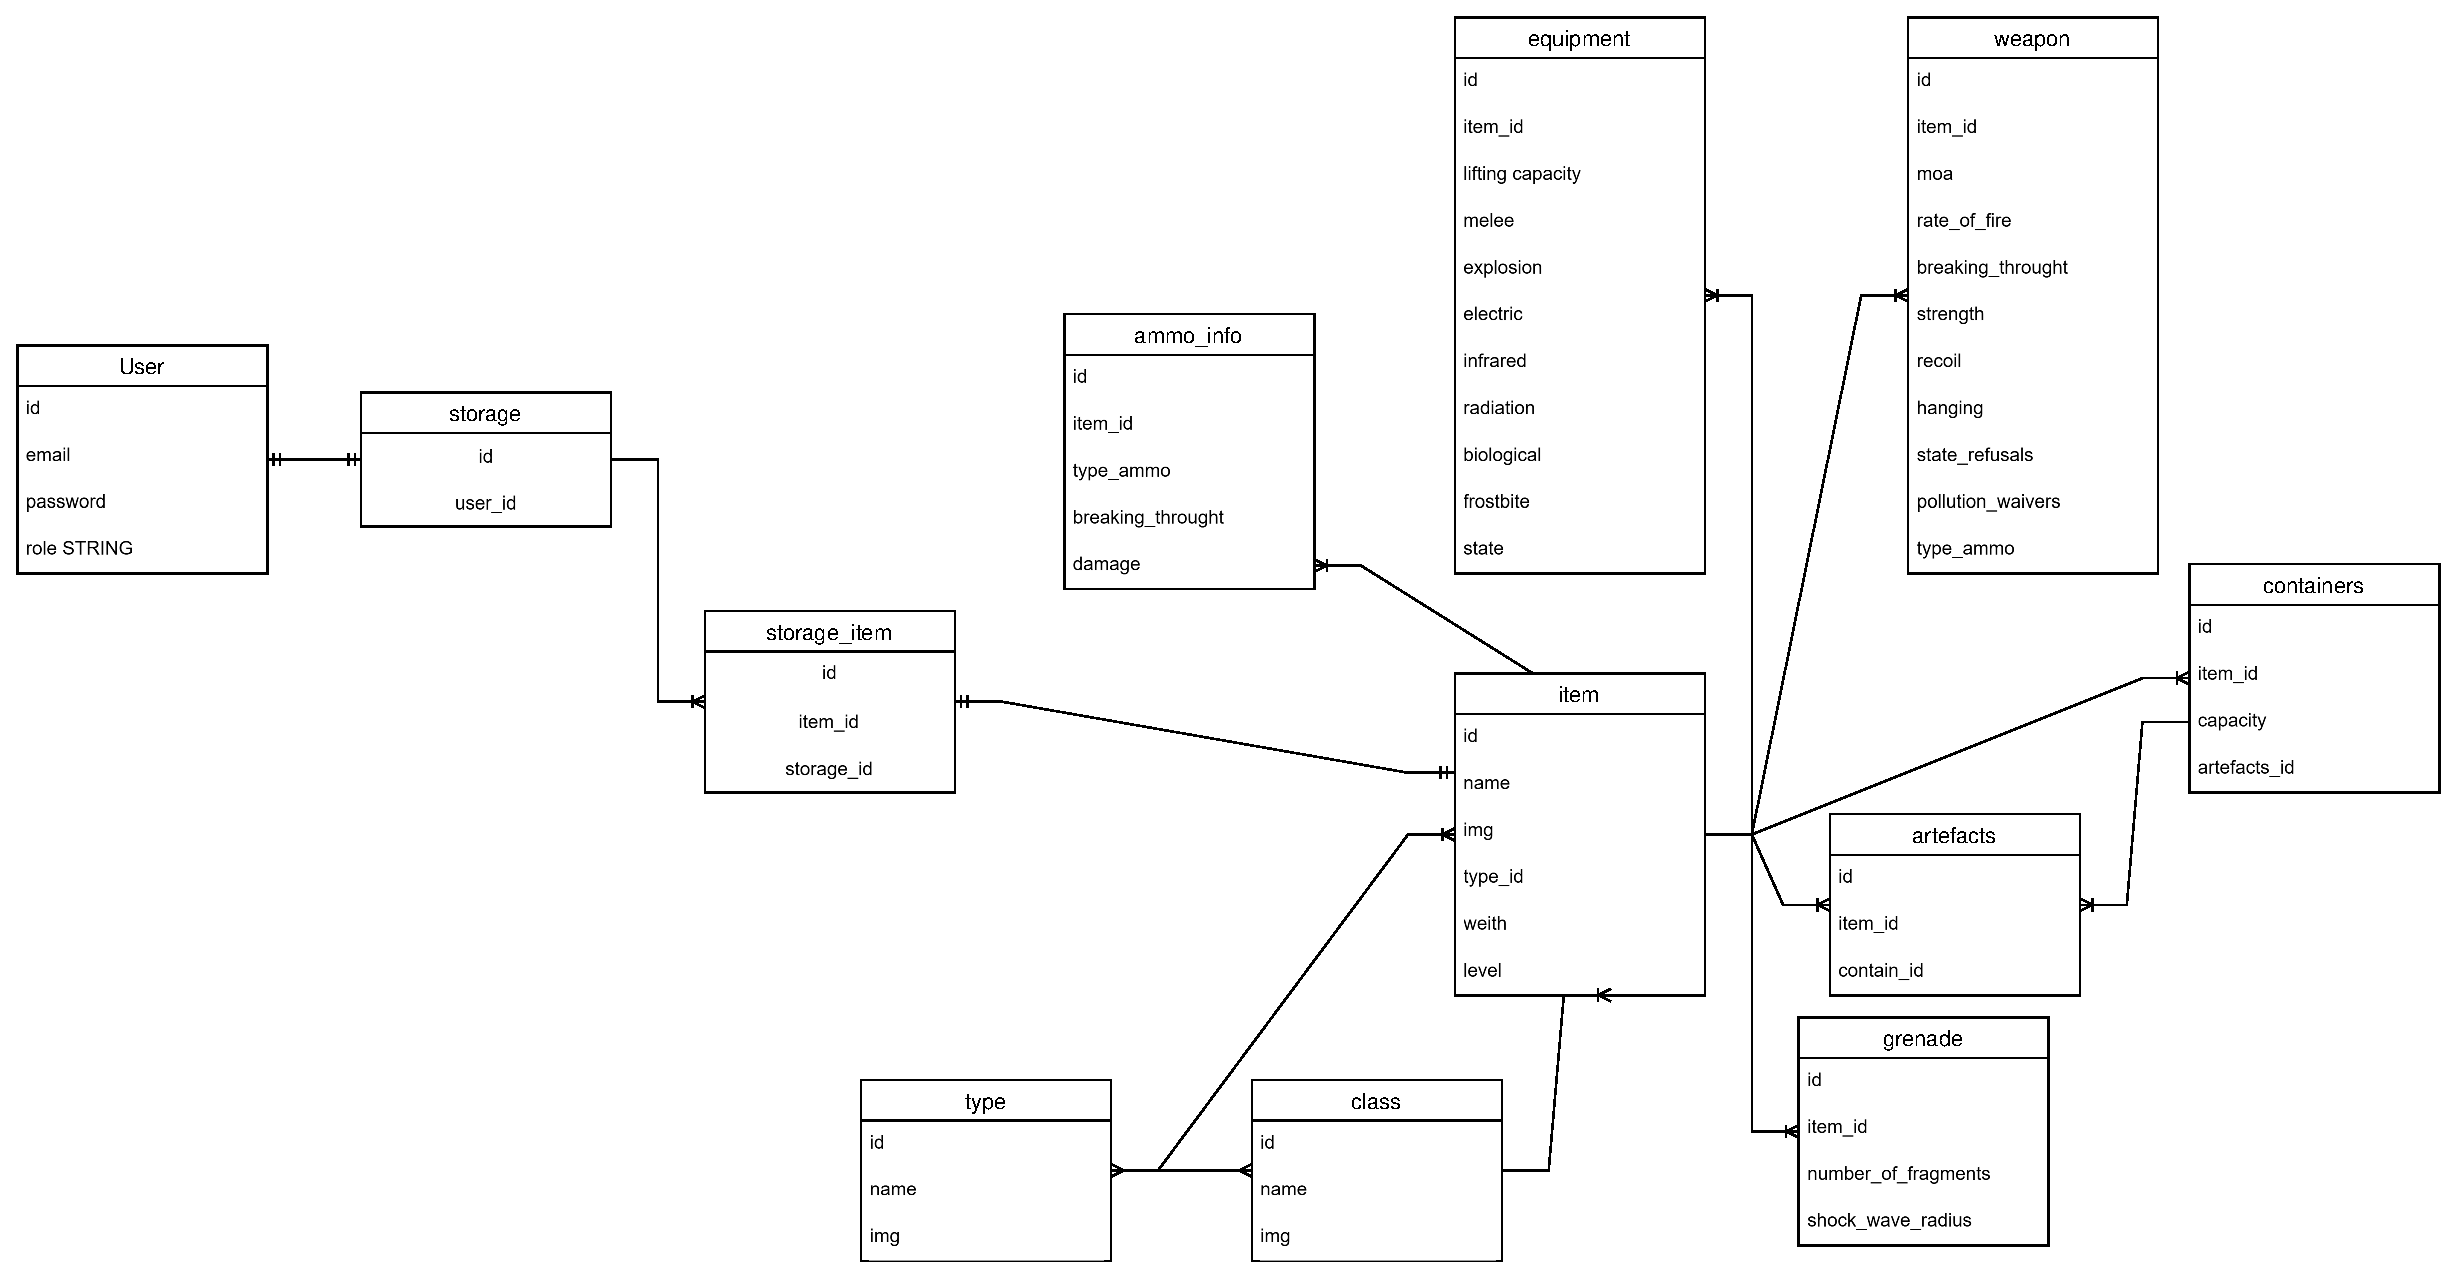
\includegraphics[width=1\linewidth]{images/modelbd}
	\caption{Концептуальная диаграмма "сущность-связь"}
	\label{fig:modelbd}
\end{figure}
%\vspace{-\figureaboveskip} % двойной отступ не нужен (можно использовать, если раздел заканчивается картинкой)

Система должна поддерживать добавление и редактирование характеристик оружия, снаряжения, боеприпасов и других категорий предметов. Также она должна обеспечивать возможность быстрого редактирования существующих предметов для отображения актуальной информации о товарах.

\subsubsection{Функциональные требования к программной системе}

В разрабатываемой программной системе должны быть реализованы следующие функции:

\begin{enumerate}
	\item Регистрация и аутентификация пользователей.
	\item Выбор сервера для торговли.
	\item Просмотр ассортимента.
	\item Просмотр информации об аккаунте.
	\item Администрирование системы.
\end{enumerate}

Диаграмма прецедентов представлена на рисунке ~\ref{fig:precendent}.

\begin{figure}[h]
	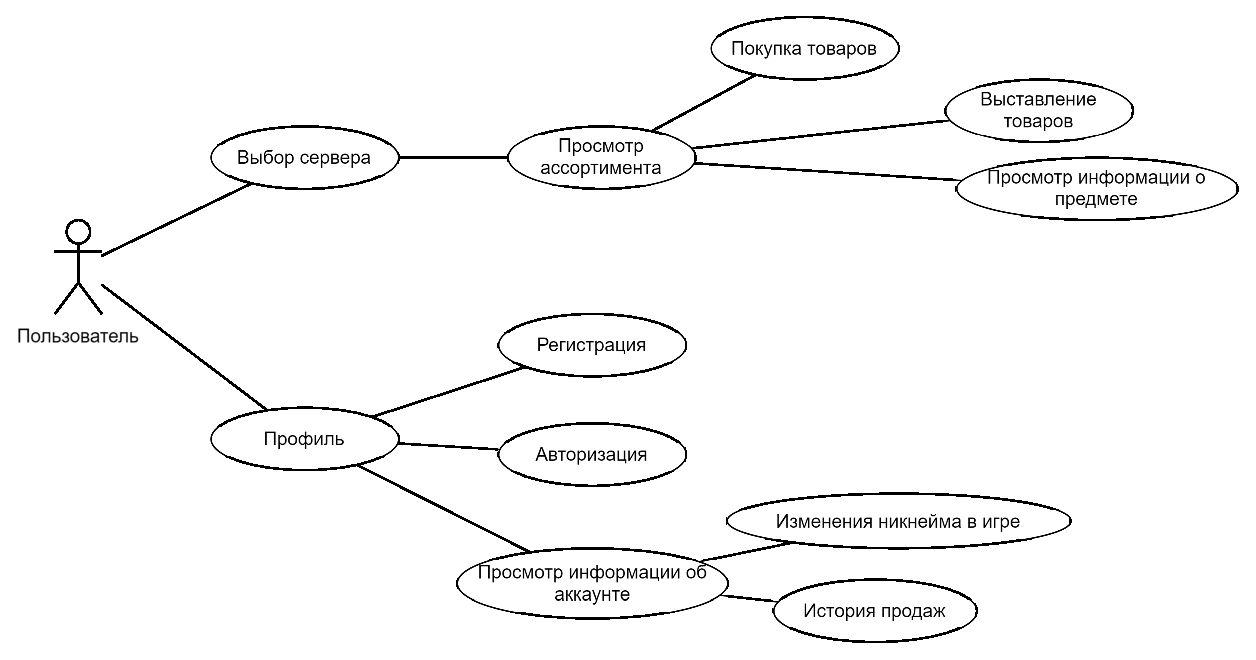
\includegraphics[width=1\linewidth]{images/precendent}
	\caption{Диаграмма прецедентов}
	\label{fig:precendent}
\end{figure}

\paragraph{Вариант использования «Выбор сервера»}

Заинтересованные лица и их требования: пользователь желает начать производить какие-либо действия на сайте, связанные с торговлей. Предусловие: открыта главная страница сайта. Постусловие: открывается нужная страница в соответствие с выбранным сервером. Основной успешный сценарий:

\begin{enumerate}
	\item Пользователь нажимает на кнопку выбора сервера на главной странице сайта.
	\item На сайте открывается модальное окно с доступными серверами.
	\item Пользователь выбирает нужный ему сервер.
	\item Приложение открывает страницу, соответствующую выбранному серверу.
\end{enumerate}

\paragraph{Вариант использования «Просмотр информации о товаре»}

Заинтересованные лица и их требования: пользователь желает получить больше информации о конкретном товаре. Предусловие: открыта страница какого-либо сервера. Постусловие: появляется модальное окно с полной информацией о товаре. Основной успешный сценарий:

\begin{enumerate}
	\item Пользователь нажимает на значок с изображением нужного товара.
	\item Приложение получает уникальный id предмета и отправляет запрос на сервер.
	\item Сервер формирует запрос в базу данных и передает данные в приложение.
	\item Приложение получает информацию от сервера и заполняет модальное окно в соответствие с полученной информацией.
\end{enumerate}

\paragraph{Вариант использования «Покупка товара»}

Заинтересованные лица и их требования: пользователь увидел интересующий его товар и захотел его приобрести. Предусловие: открыта страница какого-либо сервер. Постусловие: появляется уникальное сообщение, которое нужно скопировать и вставить в игре. Основной успешный сценарий:

\begin{enumerate}
	\item Пользователь нажимает на кнопку «Купить».
	\item  Приложение генерирует уникальное сообщение в соответствие с названием товаров и игровым никнеймом пользователя.
\end{enumerate}

\paragraph{Вариант использования «Регистрация»}

Заинтересованные лица и их требования: пользователь хочет создать свой аккаунт на сайте. Предусловие: пользователь еще не авторизовался на сайте. Постусловие: регистрация произведена, появляется значек с изображение профиля. Основной успешный сценарий:

\begin{enumerate}
	\item Пользователь нажимает на кнопку «Регистрация».
	\item Открывается экран регистрации пользователя.
	\item Пользователь вводит почту, логин, пароль и повторный пароль.
	\item Приложение отправляет запрос на сервер.
	\item Сервер формирует запрос в базу данных на создание аккаунта.
	\item Если аккаунта с таким же логином или почтой не существует, создается новый аккаунт.
	\item Сервер передает информацию в приложение о результате создания аккаунта.
	\item Приложение открывает окно пользователю с результатами регистрации.
\end{enumerate}

\paragraph{Вариант использования «Авторизация»}

Заинтересованные лица и их требования: пользователь хочет войти в свой аккаунт на сайте. Предусловие: пользователь еще не авторизовался на сайте. Постусловие: авторизация произведена, появляется значок с изображение профиля. Основной успешный сценарий:

\begin{enumerate}
	\item Пользователь нажимает на кнопку «Авторизация».
	\item Открывается экран авторизации пользователя.
	\item Пользователь вводит почту, логин, пароль и повторный пароль.
	\item Приложение отправляет запрос на сервер.
	\item Сервер формирует запрос в базу данных.
	\item База данных возвращает результат о совпадении логина и пароля.
	\item Сервер передает информацию в приложение о результате авторизации.
	\item Приложение открывает окно пользователю с результатами авторизации.
\end{enumerate}

\paragraph{Вариант использования «Выставление товара»}

Заинтересованные лица и их требования: пользователь хочет продать какую-либо вещь. Предусловие: пользователь выбрал сервер и авторизовался. Постусловие: предмет добавляется в ленту товаров:

\begin{enumerate}
	\item Пользователь нажимает на элемент интерфейса (значок с изображением плюса).
	\item Приложение открывает модальное окно с полями ввода.
	\item Пользователь вводит название предмета полностью или его часть.
	\item Приложение выводит все совпадения.
	\item Пользователь выбирает нужный ему предмет.
	\item Приложение отправляет запрос на сервер.
	\item Сервер формирует запрос в базу данных на получения все характеристик предмета.
	\item Сервер передает данные в приложение.
	\item Приложение заполняет необходимые данные в соответствие с данными.
	\item Пользователь вводит недостающие данные и выставляет предмет на продажу.
	\item Приложение отправляет запрос на сервер.
	\item Сервер вносит данные в базу данных.
	\item Сервер передает информацию о результате приложению.
	\item Приложение оповещает пользователя об успехе выставления предмета на продажу.
\end{enumerate}

\paragraph{Вариант использования «Изменение пароля»}

Заинтересованные лица и их требования: пользователь хочет поменять свой пароль на аккаунте. Предусловие: пользователь авторизировался. Постусловие: изменение пароля:

\begin{enumerate}
	\item Пользователь нажимает на кнопку "Изменить пароль"
	\item Приложение открывает модальное окно с полями ввода.
	\item Пользователь вводит текущий пароль, новый пароль повторный новый пароль.
	\item Приложение отправляет запрос на сервер.
	\item Сервер формирует запрос в базу данных на смену пароля.
	\item Сервер передает данные в приложение.
	\item Приложение оповещает пользователя об успехе выставления предмета на продажу.
\end{enumerate}

\subsubsection{Требования пользователя к интерфейсу приложения}

На сайте должны быть реализованы следующие страницы:

\begin{enumerate}
	\item Страница «Выбор сервера» -- главная страница при открытии сайта, где отображается основной текст и возможность выбрать основной сервер для торговли.
	\item Страница «Лента товаров» -- страница, на которой отображаются все товары, выставленные другими пользователями в рамках выбранного сервера в соответствии с установленными параметрами фильтрации.
	\item Страница «Профиль» -- страница для просмотра и изменения данных аккаунта.
	\item Страница «Аутентификация» -- страница, на которой пользователь может создать новый аккаунт или зайти уже в существующий.
	\item Страница «Админ панель» - страница для особой категории пользователей, являющихся администраторами на сайте, для удобного добавления новых типов, классов и предметов.
	\item Страница «Ваши товары» -- страница, на которой отображаются все товары, выставленные авторизованным пользователем, позволяет изменять состояние предмета, будь то удаление, добавление или изменение.
	\item Страница «Информация о товаре» -- страница, на которой отображается информация о выбранном товаре.
\end{enumerate}

Помимо перечисленных страниц, на сайте должны быть реализованы следующие компоненты:

\begin{itemize}
	\item окно изменения пароля;
	\item окно создания классов;
	\item окно созадния типов;
	\item окно создания предметов;
	\item окно выбора серверов;
\end{itemize}

\subsubsection{Нефункциональные требования к программной системе}

\paragraph{Требования к надежности}

В процессе использования маркетплейса могут произойти различные аварийные ситуации. Для обеспечения устойчивости и защиты данных сайт должен соответствовать следующим требованиям:

\begin{itemize}
	\item система должна работать безотказно и минимизировать время простоя;
	\item система должна быть устойчивой к аппаратным и программным сбоям;
	\item обеспечение устойчивости системы при большом количестве одновременно активных сессий пользователей;
	\item обновления системы не должны нарушать работу существующих функций и данных.
\end{itemize}

\paragraph{Требования к безопасности}

Безопасность пользователя и его данных является очень важным фактом. Для обеспечения безопасного использования необходимо учитывать следующие требования к безопасности:

\begin{itemize}
	\item пароли пользователей должны храниться в зашифрованном виде, используя современные методы хеширования;
	\item регулярное обновление программного обеспечения для устранения известных уязвимостей;
	\item регулярное создание резервных копий всех критических данных и их безопасное хранение;
	\item предоставление пользователям рекомендаций и напоминаний по обеспечению безопасности их учетных записей;
	\item обеспечение быстрого оповещения пользователей и администраторов о возможных инцидентах.
\end{itemize}

\subsection{ Требования к программному обеспечению}

Для реализации программной системы должны быть использованы следующие языки программирования:

\begin{itemize}
	\item JavaScript - серверная часть приложения;
	\item JavaScript - клиентская часть приложения;
	\item SQL для запросов к базе данных.
	\item Рабочий проект.
\end{itemize}

Для доступа к клиентской части требуется веб-браузер с поддержкой
JavaScript стандарта ECMAScript 2015.

\subsection{Требования к оформлению документации}

Требования к стадиям разработки программ и программной документации для вычислительных машин, комплексов и систем независимо от их назначения и области применения, этапам и содержанию работ устанавливаются ГОСТ 19.102–77 и ГОСТ 34.601-90.

Программная документация должна включать в себя:

\begin{itemize}
	\item Анализ предметной области.
	\item Техническое задание.
	\item Технический проект.
	\item Рабочий проект.
\end{itemize}

\section{Технический проект}
\subsection{Общая характеристика организации решения задачи}

Необходимо спроектировать и разработать сайт, который должен способствовать упрощению реализации цифровых предметов внутри игры «Stay Out».

Веб-сайт представляет собой набор взаимосвязанных электронных страниц, объединенных в логическую структуру и содержащих различные виды контента: текст, графику и мультимедийные элементы. Сайт разработан с использованием таких технологий, как HTML, CSS и JavaScript.

Разрабатываемый веб-сайт будет предоставлять пользователям возможность создания учетных записей, выставления и поиска внутриигровых ценностей, а также обмена ими с другими игроками. Он будет обеспечивать удобный интерфейс для взаимодействия между игроками, обеспечивая прозрачность и безопасность сделок.

\subsection{Обоснование выбора технологии проектирования}

Используемые для создания программно-информационной системы языки и технологии отвечают современным практикам разработки, позволяют достичь высокой производительности и отказоустойчивости программы.

\subsubsection{Описание используемых технологий и языков программирования}

В процессе разработки web-сайта используются программные средства и языки программирования. Каждое программное средство и каждый язык программирования применяется для круга задач, при решении которых они необходимы.

\subsubsection{Язык программирования JavaScript}

JavaScript - это интерпретируемый, объектно-ориентированный язык программирования, который широко используется для создания интерактивных и динамических веб-сайтов. Благодаря своей многофункциональности, JavaScript является одним из самых популярных языков программирования в мире веб-разработки.

В отличие от многих других языков программирования, JavaScript выполняется непосредственно в веб-браузере пользователя. Это позволяет ему взаимодействовать с элементами HTML страницы, управлять их содержимым, изменять стили, реагировать на пользовательские действия и многое другое, что делает веб-страницы более интерактивными и динамичными.

JavaScript широко используется для разработки различных веб-приложений, таких как интерфейсы пользователя, игры, анимации, формы обратной связи, веб-сервисы и многое другое. Благодаря своей популярности и гибкости, JavaScript также стал широко используемым для разработки серверной стороны приложений с использованием платформы Node.js.

Язык JavaScript имеет динамическую типизацию данных, что означает, что переменные не требуют явного объявления типа данных, и их тип может изменяться в процессе выполнения программы. Это делает JavaScript гибким и удобным для быстрой разработки прототипов и простых скриптов.

Важно отметить, что JavaScript не следует путать с языком Java, несмотря на сходство в названиях. JavaScript и Java - это разные языки программирования с разными синтаксисами, целями и областями применения. JavaScript был создан компанией Netscape в начале 1990-х годов и был изначально разработан для управления взаимодействием с пользователем на веб-страницах.

На сегодняшний день JavaScript является основным инструментом для создания интерактивных элементов на веб-страницах, таких как всплывающие окна, обновление данных без перезагрузки страницы (через AJAX), обработка событий от пользователя и многие другие. Современные фреймворки и библиотеки, такие как React, Angular и Vue.js, значительно упрощают и ускоряют процесс разработки сложных веб-приложений, предоставляя разработчикам мощные инструменты для создания высококачественных интерфейсов.

Кроме того, с развитием технологий JavaScript начал использоваться не только на стороне клиента, но и на стороне сервера. Платформа Node.js позволяет выполнять JavaScript код на сервере, что открывает новые возможности для создания масштабируемых и высокопроизводительных серверных приложений. Это делает JavaScript универсальным языком программирования, применимым как для клиентской, так и для серверной части веб-разработки.

\subsubsection{Библиотека React JS}

React -- это библиотека JavaScript с открытым кодом для создания внешних пользовательских интерфейсов. В отличие от других библиотек JavaScript, предоставляющих полноценную платформу приложений, React ориентируется исключительно на создание представлений приложений через инкапсулированные единицы (называются компонентами), которые сохраняют состояние и генерируют элементы пользовательского интерфейса. В React свойства передаются от родительских компонентов к дочерним. Компоненты получают свойства неизменяемых значений, из-за чего компонент не может напрямую изменять свойства, но может вызывать изменения через callback-функции.

\subsubsection{Фреймворк JS Express}

Express -- это фреймворк, написанный на языке JavaScript, который применяется в разработке бизнес-логики мобильных приложений и сайтов. Поскольку пользовательская часть сайтов работает исключительно на JavaScript, использование Express в качестве фреймворка позволяет задействовать JavaScript в пользовательской и серверной части веб-приложения.

\subsubsection{PostgreSQL}

PostgreSQL -- это объектно-реляционная система управления базами данных, основанная на POSTGRES - программе, разработанной на факультете компьютерных наук Калифорнийского университета в Беркли. У нее множество преимуществ, очень важным из которых является возможность установить СУБД на любую операционную систему, к тому же она бесплатная, что на том же MacOS является довольно важным критерием.

\subsubsection{Архитектура программной системы}

Разрабатываемая программная система основывается на клиент-серверной модели, которая является широко используемой парадигмой для разработки распределенных приложений. Эта модель позволяет распределять задачи и ответственность между несколькими компонентами, обеспечивая гибкость, масштабируемость и упрощение обслуживания. Клиентская часть системы является интерфейсом, с которым взаимодействует пользователь. Клиент выполняет функции отображения данных и приема ввода от пользователя. Серверная часть системы является компонентом, который обрабатывает запросы от клиентов, выполняет основную бизнес-логику и управляет данными. Сервер может быть размещен на мощных вычислительных платформах, обеспечивающих высокую производительность и надежность.

\subsection{Диаграмма компонентов}

Диаграмма компонентов является важным инструментом для описания физического представления разрабатываемой системы. Она позволяет разработчикам определить архитектуру системы, выявив взаимосвязи и зависимости между программными компонентами, включая как исходный, так и исполняемый код.

Основными элементами диаграммы компонентов являются компоненты, интерфейсы и зависимости между ними. Компоненты представляют собой логические единицы функциональности системы, которые могут быть как отдельными приложениями, так и более крупными модулями или сервисами.

\begin{figure}[h]
	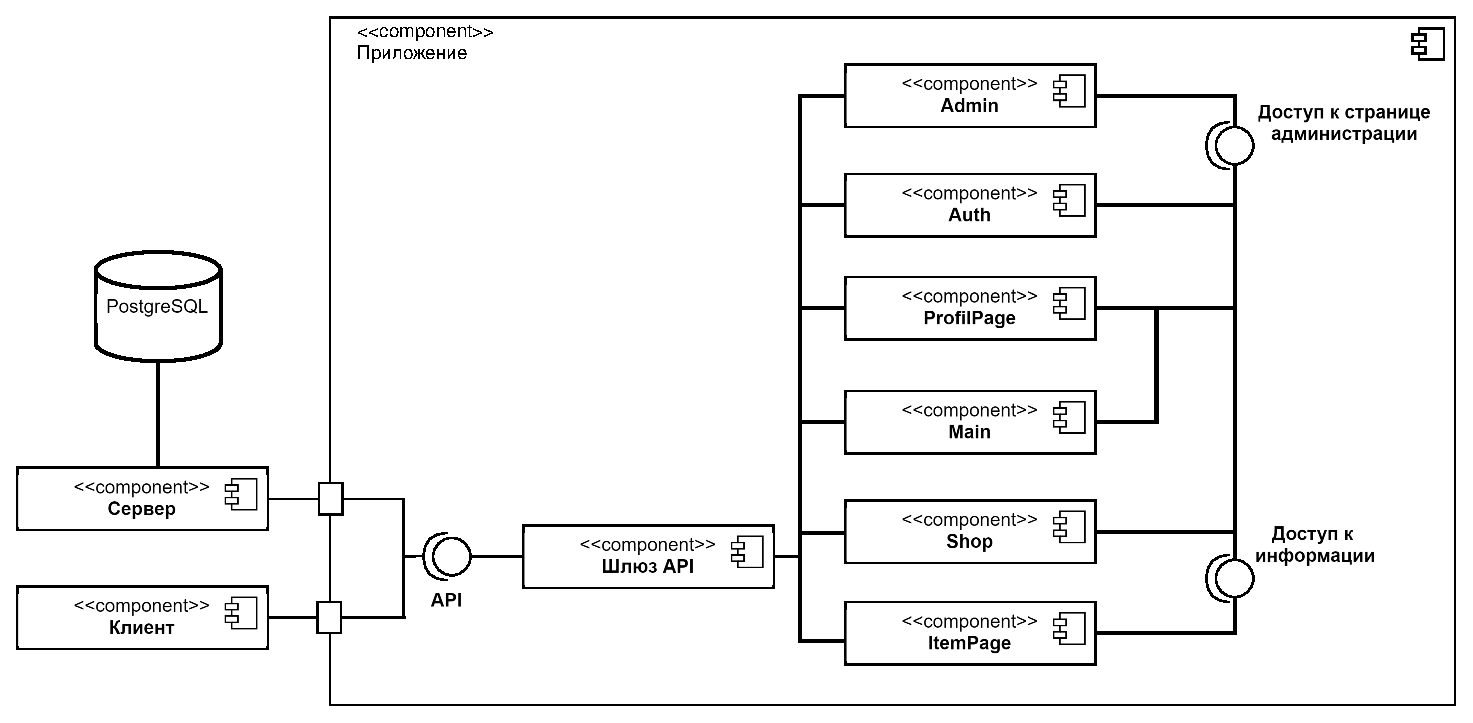
\includegraphics[width=1\linewidth]{images/diagcomp}
	\caption{Диаграмма компонентов}
	\label{fig:diagcomp}
\end{figure}

Интерфейсы определяют способы взаимодействия между компонентами, задавая набор методов, сообщений или протоколов, которыми компоненты обмениваются информацией.

Зависимости указывают на связи между компонентами, определяя порядок и направление потока данных или контроля между ними.

На рисунке \ref{fig:diagcomp} представлена диаграмма компонентов для проектируемой системы.

\subsection{Диаграмма размещения}

Диаграмма размещения используется для визуализации физического расположения компонентов программной системы на аппаратных платформах. Она является важным инструментом в процессе проектирования и реализации программного обеспечения, так как позволяет показать, как различные части системы будут распределены по различным узлам (например, серверам, компьютерам, сетевому оборудованию). Диаграмма размещения помогает архитекторам и разработчикам понять физическое развертывание системы, а также определить, какие узлы будут взаимодействовать друг с другом и каким образом.

На рисунке \ref{fig:diagrazm} представлена диаграмма размещения для проектируемой системы.

\vspace{-8mm} % чтобы убрать пустую строку, которая осталась после переноса рисунка на следующую страницу
\begin{figure}[h]
	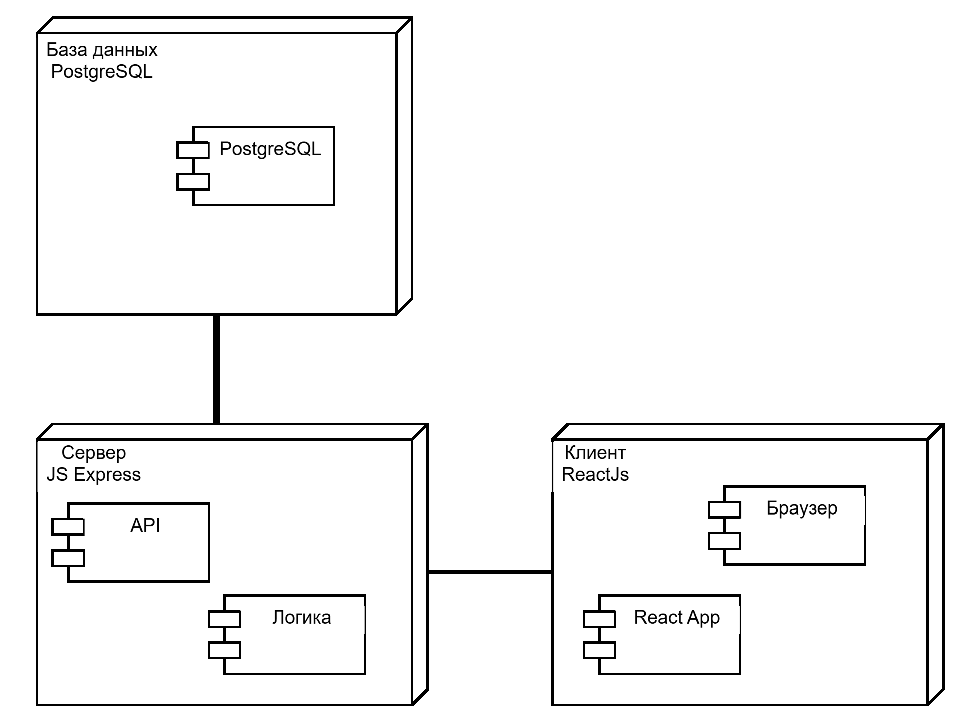
\includegraphics[width=0.5\linewidth]{images/diagrazm}
	\caption{Диаграмма размещения}
	\label{fig:diagrazm}
\end{figure}

\subsection{Конечные точки серверной части}

Для организации взаимодействия клиентской части с бизнес-логикой приложения были определены конечные точки. На рисунке \ref{fig:routes} представлена карта маршрутов, представляющее схематическое изображение конечных точек.

\begin{figure}
	\centering
	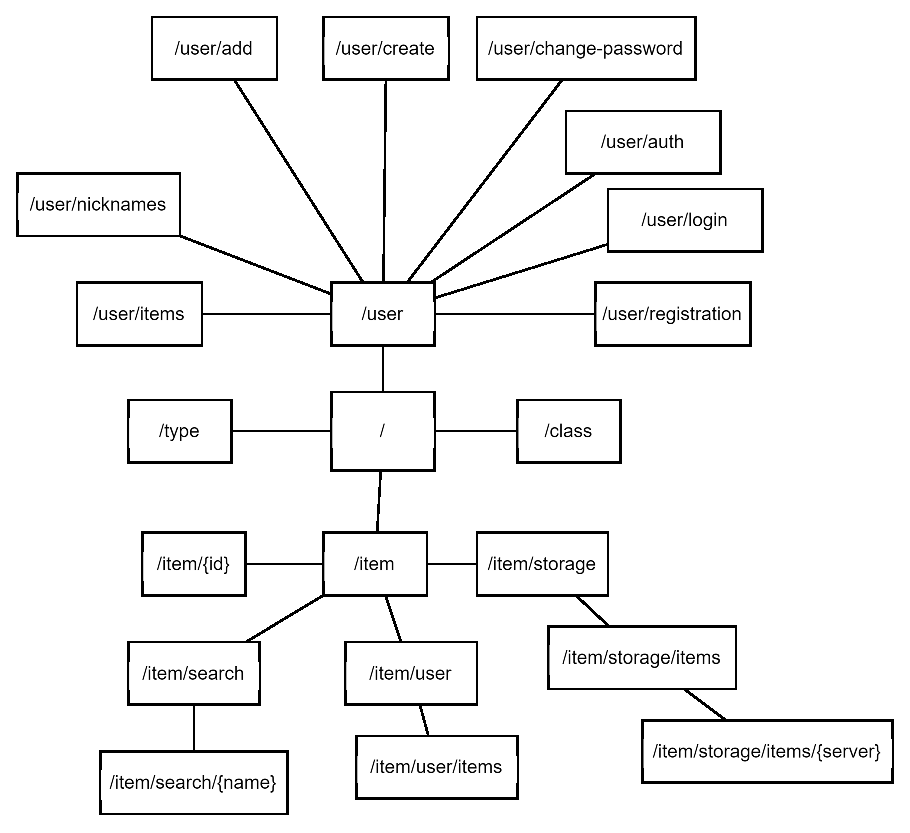
\includegraphics[width=0.7\linewidth]{images/routes}
	\caption{Карта маршрутов}
	\label{fig:routes}
\end{figure}

POST /user/registration - Регистрация нового пользователя.

POST /user/login - Вход пользователя в систему.

GET /user/auth - Проверка авторизации пользователя.

POST /user/change-password - Изменение пароля пользователя.

POST /user/create - Создание хранилища для пользователя.

POST /user/add - Добавление предмета в хранилище пользователя.

GET /user/items - Получение предметов из хранилища пользователя.

PUT /user/nicknames - Обновление никнеймов пользователя.

POST /class/ - Создание нового класса предмета.

GET /class/ - Получение всех классов предметов.

POST /type/ - Создание нового типа предмета.

GET /type/ - Получение всех типов предметов.

POST /item/ - Создание нового предмета.

GET /item/ - Получение всех предметов с возможностью фильтрации.

GET /item/:id - Получение конкретного предмета по его ID.

GET /item/search/:name - Поиск предметов по имени.

GET /item/storage/items/:server - Получение предметов из хранилища по серверу.

POST /item/storage/add - Добавление предмета в хранилище.

GET /item/user/items - Получение предметов пользователя.

DELETE /item/:id - Удаление предмета по его ID.

GET /item/ammo\_infos/:itemId - Получение информации о боеприпасах по ID предмета.

\subsection{Проект данных программной системы}

Согласно требованиям технического задания, веб-сайт должен взаимодействовать с двумя базами данных.

На серверной стороне предполагается использование PostgreSQL, реляционной базы данных, которая обеспечивает хранение структурированных данных.

Для веб-сайта предусмотрено использование локального хранилища localStorage для хранения JWT токена, что позволяет сайту сохранять информацию о сессии пользователя между сеансами.

Реляционные базы данных, такие как PostgreSQL, используют таблицы для хранения данных в структурированном формате и оперируют ими с помощью SQL. Этот подход обеспечивает надежность и консистентность данных.

Использование localStorage для хранения JWT токена позволяет сайту сохранять и использовать информацию о пользовательской сессии без необходимости подключения к сети, что улучшает пользовательский опыт и обеспечивает безопасность данных.

\subsection{Описание сущностей серверной части}

В состав сущности "<Пользователь"> можно включить атрибуты, представленные в таблице \ref{news:table}.

\begin{xltabular}{\textwidth}{|l|l|p{1.7cm}|X|}
	\caption{Атрибуты сущности "<Пользователь">\label{news:table}}\\ \hline
	\centrow Поле & \centrow Тип & \centrow Обяза\-тельное & \centrow Описание \\ \hline
	\thead{1} & \thead{2} & \centrow 3 & \centrow 4 \\ \hline
	\endfirsthead
	\continuecaption{Продолжение таблицы \ref{news:table}}
	\thead{1} & \thead{2} & \centrow 3 & \centrow 4 \\ \hline
	\finishhead
	id & ObjectId & true & Уникальный идентификатор \\ \hline 
	email & String & true & Почта \\ \hline 
	login & String & true & Псевдоним \\ \hline
	password & String & true & Пароль \\ \hline 
	role & String & true & Привилегия \\ \hline 
	status & String & true & Статус \\ \hline 
\end{xltabular}

В состав сущности "<Предметы"> можно включить атрибуты, представленные в таблице \ref{proda:table}.

\begin{xltabular}{\textwidth}{|R|C{2.5cm}|l|T|}
	\caption{Атрибуты  сущности "<Предметы"> с использованием различных типов столбцов и многострочным заголовком\label{proda:table}}\\ \hline
	\centrow Поле & \centrow Тип & \centrow Обязательное & \centrow Описание \\ \hline
	\centrow 1 & \centrow 2 & \thead{3} & \centrow 4 \\ \hline
	\endfirsthead
	\continuecaption{Продолжение таблицы \ref{proda:table}}
	\centrow 1 & \centrow 2 & \thead{3} & \centrow 4 \\ \hline
	\finishhead
	id & ObjectId & true & Уникальный идентификатор \\ \hline 
	name & String & true & Название \\ \hline 
	description & String & false & Описание \\ \hline 
	img & String & true & Путь до изображения \\ \hline 
	weight & String & true & Вес \\ \hline 
	level & String & true & Уровень \\ \hline 
\end{xltabular}

В состав сущности "<Тип"> можно включить атрибуты, представленные в таблице \ref{prod1:table}.

\begin{xltabular}{\textwidth}{|R|C{2.5cm}|l|T|}
	\caption{Атрибуты  сущности "<Тип"> с использованием различных типов столбцов и многострочным заголовком\label{prod1:table}}\\ \hline
	\centrow Поле & \centrow Тип & \centrow Обязательное & \centrow Описание \\ \hline
	\centrow 1 & \centrow 2 & \thead{3} & \centrow 4 \\ \hline
	\endfirsthead
	\continuecaption{Продолжение таблицы \ref{prod1:table}}
	\centrow 1 & \centrow 2 & \thead{3} & \centrow 4 \\ \hline
	\finishhead
	id & ObjectId & true & Уникальный идентификатор \\ \hline 
	name & String & true & Название \\ \hline 
	img & String & true & Путь до изображения \\ \hline 
\end{xltabular}

В состав сущности "<Класс"> можно включить атрибуты, представленные в таблице \ref{prod2:table}.

\begin{xltabular}{\textwidth}{|R|C{2.5cm}|l|T|}
	\caption{Атрибуты  сущности "<Класс"> с использованием различных типов столбцов и многострочным заголовком\label{prod2:table}}\\ \hline
	\centrow Поле & \centrow Тип & \centrow Обязательное & \centrow Описание \\ \hline
	\centrow 1 & \centrow 2 & \thead{3} & \centrow 4 \\ \hline
	\endfirsthead
	\continuecaption{Продолжение таблицы \ref{prod2:table}}
	\centrow 1 & \centrow 2 & \thead{3} & \centrow 4 \\ \hline
	\finishhead
	id & ObjectId & true & Уникальный идентификатор \\ \hline 
	name & String & true & Название \\ \hline 
	img & String & true & Путь до изображения \\ \hline 
\end{xltabular}

В состав сущности "<Экипировка"> можно включить атрибуты, представленные в таблице \ref{prod3:table}.

\begin{xltabular}{\textwidth}{|R|C{2.5cm}|l|T|}
	\caption{Атрибуты  сущности "<Экипировка"> с использованием различных типов столбцов и многострочным заголовком\label{prod3:table}}\\ \hline
	\centrow Поле & \centrow Тип & \centrow Обязательное & \centrow Описание \\ \hline
	\centrow 1 & \centrow 2 & \thead{3} & \centrow 4 \\ \hline
	\endfirsthead
	\continuecaption{Продолжение таблицы \ref{prod3:table}}
	\centrow 1 & \centrow 2 & \thead{3} & \centrow 4 \\ \hline
	\finishhead
	id & ObjectId & true & Уникальный идентификатор \\ \hline 
	lifting\_capacity & String & true & Грузоподъемность \\ \hline 
	melee & String & true & Рукопашная \\ \hline 
	explosion & String & true & Взрыв \\ \hline
	electric & String & true & Электрическое \\ \hline 
	infrared & String & true & Инфракрасное \\ \hline 
	radiation & String & true & Радиация \\ \hline 
	biological & String & true & Биологическое \\ \hline 
	frostbite & String & true & Обморожение \\ \hline 
	state & String & true & Состояние \\ \hline 
\end{xltabular}

В состав сущности "<Патроны"> можно включить атрибуты, представленные в таблице \ref{prod4:table}.

\begin{xltabular}{\textwidth}{|R|C{2.5cm}|l|T|}
	\caption{Атрибуты  сущности "<Патроны"> с использованием различных типов столбцов и многострочным заголовком\label{prod4:table}}\\ \hline
	\centrow Поле & \centrow Тип & \centrow Обязательное & \centrow Описание \\ \hline
	\centrow 1 & \centrow 2 & \thead{3} & \centrow 4 \\ \hline
	\endfirsthead
	\continuecaption{Продолжение таблицы \ref{prod4:table}}
	\centrow 1 & \centrow 2 & \thead{3} & \centrow 4 \\ \hline
	\finishhead
	id & ObjectId & true & Уникальный идентификатор \\ \hline 
	type\_ammo & String & true & Тип \\ \hline 
	breaking\_throught & String & true & Пробитие \\ \hline 
	damage & String & true & Урон \\ \hline 
\end{xltabular}

В состав сущности "<Оружие"> можно включить атрибуты, представленные в таблице \ref{prod5:table}.

\begin{xltabular}{\textwidth}{|R|C{2.5cm}|l|T|}
	\caption{Атрибуты  сущности "<Оружие"> с использованием различных типов столбцов и многострочным заголовком\label{prod5:table}}\\ \hline
	\centrow Поле & \centrow Тип & \centrow Обязательное & \centrow Описание \\ \hline
	\centrow 1 & \centrow 2 & \thead{3} & \centrow 4 \\ \hline
	\endfirsthead
	\continuecaption{Продолжение таблицы \ref{prod5:table}}
	\centrow 1 & \centrow 2 & \thead{3} & \centrow 4 \\ \hline
	\finishhead
	id & ObjectId & true & Уникальный идентификатор \\ \hline 
	moa & String & true & Угловая минута \\ \hline 
	rate\_of\_fire & String & true & Темп \\ \hline 
	breaking\_throught & String & true & Пробитие \\ \hline 
	strength & String & true & Прочность \\ \hline 
	recoil & String & true & Отдача \\ \hline 
	handing & String & true & Качание \\ \hline 
	rocw & String & true & Отказ от состояния \\ \hline 
	no\_pollutin & String & true & Отказ от загрязнения \\ \hline 
	type\_ammo & String & true & Тип патрона \\ \hline 
\end{xltabular}

В состав сущности "<Гранаты"> можно включить атрибуты, представленные в таблице \ref{prod6:table}.

\begin{xltabular}{\textwidth}{|R|C{2.5cm}|l|T|}
	\caption{Атрибуты  сущности "<Гранаты"> с использованием различных типов столбцов и многострочным заголовком\label{prod6:table}}\\ \hline
	\centrow Поле & \centrow Тип & \centrow Обязательное & \centrow Описание \\ \hline
	\centrow 1 & \centrow 2 & \thead{3} & \centrow 4 \\ \hline
	\endfirsthead
	\continuecaption{Продолжение таблицы \ref{prod6:table}}
	\centrow 1 & \centrow 2 & \thead{3} & \centrow 4 \\ \hline
	\finishhead
	id & ObjectId & true & Уникальный идентификатор \\ \hline 
	number\_of\_fragments & String & true & Количество осколков \\ \hline 
	shock\_wave\_radius & String & true & Радиус взрыва \\ \hline 
\end{xltabular}

В системе предусмотрен внутренний механизм связи между разделами и элементами информационных блоков, что обеспечивает эффективную организацию данных без необходимости введения дополнительных идентификаторов при реализации связей между сущностями.

Каждая сущность в системе представлена экземпляром информационного блока, который содержит элементы, отражающие конкретные атрибуты или характеристики данной сущности. Поля и свойства элементов информационных блоков служат для описания атрибутов сущности.

Благодаря этому подходу, данные о сущностях хранятся и управляются структурированно и легко доступны для обработки. Экземпляры сущностей, представленные элементами информационных блоков, обеспечивают гибкость в управлении данными, позволяя эффективно адаптировать информационную структуру системы к различным потребностям и изменениям в бизнес-логике.

Такой подход минимизирует необходимость введения дополнительных идентификаторов или средств для организации связей между сущностями, упрощая процесс разработки и поддержки системы. Кроме того, он способствует повышению производительности и надежности обработки данных, так как предусматривает оптимальное использование внутренних механизмов управления информацией.

\subsection{Проектирование пользовательского интерфейса}

На основе требований к пользовательскому интерфейсу, представленных в пункте 2.3.3 технического задания, был разработан графический интерфейс для взаимодействия с приложением. Для стилизации некоторых компонентов использовался CSS 3. Для разработки интерфейса использовалась библиотека React вместе с библиотекой React-компонентов React-Bootstrap. На представленных ниже рисунках числами обозначены элементы графического интерфейса. На рисунке \ref{fig:regmaket} представлен макет страницы регистрации пользователя. Страница регистрации содержит следующие элементы:

\begin{enumerate}
	\item Форма регистрации.
	\item Поле ввода электронной почты.
	\item Поле ввода пароля.
	\item Ссылка на форму авторизации.
	\item Кнопка подтверждения формы.
\end{enumerate}

\begin{figure}
	\centering
	
\includegraphics[width=0.7\linewidth]{images/reg_maket}
	\caption{Макет страницы регистрации}
	\label{fig:regmaket}
\end{figure}

На рисунке \ref{fig:logmaket} представлен макет страницы авторизации. Страница авторизации содержит следующие элементы:

\begin{enumerate}
	\item Форма авторизации.
	\item Поле ввода электронной почты.
	\item Поле ввода пароля.
	\item Ссылка на форму регистрации.
	\item Кнопка подтверждения формы.
\end{enumerate}

\begin{figure}
	\centering
	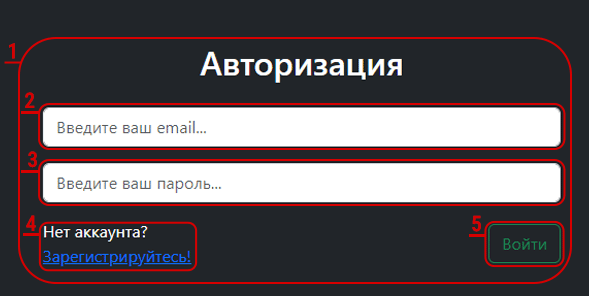
\includegraphics[width=0.7\linewidth]{images/log_maket}
	\caption{Макет страницы авторизации}
	\label{fig:logmaket}
\end{figure}

На рисунке \ref{fig:mainmaket} представлен макет главной страницы. Главная страница содержит следующие элементы:

\begin{enumerate}
	\item Ссылка на главную страницу.
	\item Кнопка вызова формы выбора сервера.
	\item Кнопка перехода на страницу администрации.
	\item Кнопка перехода в профиль.
\end{enumerate}

\begin{figure}
	\centering
	
\includegraphics[width=0.7\linewidth]{images/main_maket}
	\caption{Макет главной страницы}
	\label{fig:mainmaket}
\end{figure}

На рисунке \ref{fig:shopmaket} представлен макет страницы маркетплейса. Страница маркетплейса содержит следующие элементы:

\begin{enumerate}
	\item Ссылка на главную страницу.
	\item Тип предмета.
	\item Класс предмета.
	\item Форма предмета.
	\item Изображение предмета.
	\item Никнейм игрового персонажа.
	\item Характеристики предмета.
	\item Кнопка покупки предмета.
	\item Кнопка перехода на страницу администрации.
	\item Кнопка перехода в профиль.
	\item Отображение выбранной страницы.
	\item Кнопка выставления предмета на продажу.
\end{enumerate}

\begin{figure}
	\centering
	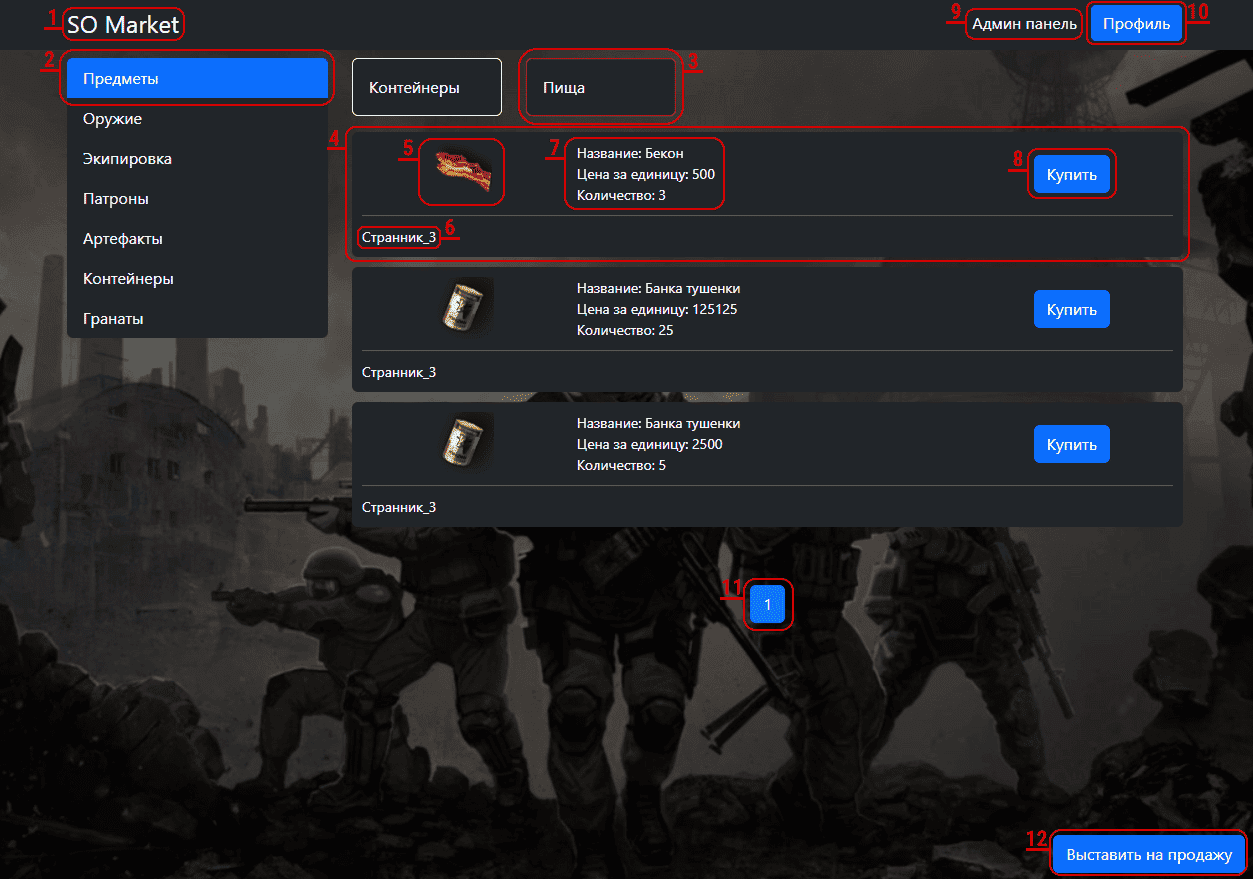
\includegraphics[width=0.7\linewidth]{images/shop_maket}
	\caption{Макет страницы магазина}
	\label{fig:shopmaket}
\end{figure}


\ifПрактика{}\else{
   \section{Рабочий проект}
\subsection{Классы, используемые при разработке сайта}

В результате разработки маркетплейса были реализованы классы и компоненты, обеспечивающие работоспособность системы. Спецификация классов и компонентов описана в этой главе. (таблица \ref{class:table}).

\subsubsection{Спецификация класса ClassController}

Этот класс предназначен для управления операциями, связанными с классами. Он включает методы для создания и получения всех классов.

\renewcommand{\arraystretch}{0.8}
\begin{xltabular}{\textwidth}{|X|p{2.5cm}|p{4.85cm}|p{4.85cm}|}
	\caption{Описание методов класса ClassController\label{classcontroller:table}}\\
	\hline Название метода & Область видимости & Тип значения & Описание \\
	\hline \endfirsthead
	\caption*{Продолжение таблицы \ref{classcontroller:table}}\\
	\hline Название метода & Область видимости & Тип значения & Описание \\
	\hline \endhead
	create & public & Promise & Создает новый класс на основе данных из тела запроса и возвращает его в формате JSON. \\
	\hline
	getAll & public & Promise & Возвращает список всех классов в формате JSON. \\
	\hline
\end{xltabular}
\renewcommand{\arraystretch}{1.0}

\subsubsection{Спецификация класса ItemController}

Этот класс управляет операциями, связанными с предметами. Он включает методы для создания, получения, поиска и удаления предметов, а также для работы с хранилищем.

\renewcommand{\arraystretch}{0.8}
\begin{xltabular}{\textwidth}{|X|p{2.5cm}|p{4.85cm}|p{4.85cm}|}
	\caption{Описание методов класса ItemController\label{itemcontroller:table}}\\
	\hline Название метода & Область видимости & Тип значения & Описание \\
	\hline \endfirsthead
	\caption*{Продолжение таблицы \ref{itemcontroller:table}}\\
	\hline Название метода & Область видимости & Тип значения & Описание \\
	\hline \endhead
	create & public & Promise & Создает новый предмет на основе данных из тела запроса и возвращает его в формате JSON. \\
	\hline
	getAll & public & Promise & Возвращает список всех предметов в формате JSON с учетом фильтров и пагинации. \\
	\hline
	getOne & public & Promise & Возвращает один предмет по его идентификатору. \\
	\hline
	search & public & Promise & Ищет предметы по их названию и возвращает результаты в формате JSON. \\
	\hline
	getStorage Items & public & Promise & Возвращает предметы из хранилища с учетом фильтров и пагинации. \\
	\hline
	getUserItems & public & Promise & Возвращает предметы пользователя из хранилища. \\
	\hline
	addItemTo Storage & public & Promise & Добавляет предмет в хранилище и возвращает его в формате JSON. \\
	\hline
	deleteItem & public & Promise & Удаляет предмет из хранилища по его идентификатору. \\
	\hline
	getAmmo InfosBy ItemId & public & Promise & Возвращает информацию о патронах для заданного предмета. \\
	\hline
\end{xltabular}
\renewcommand{\arraystretch}{1.0}

\subsubsection{Спецификация класса TypeController}

Этот класс управляет операциями, связанными с типами предметов. Он включает методы для создания и получения всех типов.

\renewcommand{\arraystretch}{0.8}
\begin{xltabular}{\textwidth}{|X|p{2.5cm}|p{4.85cm}|p{4.85cm}|}
	\caption{Описание методов класса TypeController\label{typecontroller:table}}\\
	\hline Название метода & Область видимости & Тип значения & Описание \\
	\hline \endfirsthead
	\caption*{Продолжение таблицы \ref{typecontroller:table}}\\
	\hline Название метода & Область видимости & Тип значения & Описание \\
	\hline \endhead
	create & public & Promise & Создает новый тип предмета на основе данных из тела запроса и возвращает его в формате JSON. \\
	\hline
	getAll & public & Promise & Возвращает список всех типов предметов в формате JSON. \\
	\hline
\end{xltabular}
\renewcommand{\arraystretch}{1.0}

\subsubsection{Спецификация класса UserController}

Этот класс управляет операциями, связанными с пользователями. Он включает методы для регистрации, аутентификации, изменения пароля и управления хранилищем.

\renewcommand{\arraystretch}{0.8}
\begin{xltabular}{\textwidth}{|X|p{2.5cm}|p{4.85cm}|p{4.85cm}|}
	\caption{Описание методов класса UserController\label{usercontroller:table}}\\
	\hline Название метода & Область видимости & Тип значения & Описание \\
	\hline \endfirsthead
	\caption*{Продолжение таблицы \ref{usercontroller:table}}\\
	\hline Название метода & Область видимости & Тип значения & Описание \\
	\hline \endhead
	registration & public & Promise & Регистрация нового пользователя с хешированным паролем и создание для него хранилища. \\
	\hline
	login & public & Promise & Аутентификация пользователя и генерация JWT токена. \\
	\hline
	check & public & Promise & Проверка JWT токена пользователя. \\
	\hline
	change Password & public & Promise & Изменение пароля пользователя. \\
	\hline
	createStorage & public & Promise & Создание нового хранилища для пользователя. \\
	\hline
	addItemTo Storage & public & Promise & Добавление предмета в хранилище пользователя. \\
	\hline
	getItems FromStorage & public & Promise & Получение предметов из хранилища с учетом фильтров и пагинации. \\
	\hline
	update Nicknames & public & Promise & Обновление никнеймов пользователя. \\
	\hline
\end{xltabular}
\renewcommand{\arraystretch}{1.0}

\subsubsection{Спецификация класса ItemStore}

Этот класс управляет состоянием предметов и их типов в приложении. Он включает методы для установки и получения типов, классов и предметов, а также для управления пагинацией.

\renewcommand{\arraystretch}{0.8}
\begin{xltabular}{\textwidth}{|X|p{2.5cm}|p{4.85cm}|p{4.85cm}|}
	\caption{Описание методов класса ItemStore\label{itemstore:table}}\\
	\hline Название метода & Область видимости & Тип значения & Описание \\
	\hline \endfirsthead
	\caption*{Продолжение таблицы \ref{itemstore:table}}\\
	\hline Название метода & Область видимости & Тип значения & Описание \\
	\hline \endhead
	setTypes & public & void & Устанавливает список типов предметов. \\
	\hline
	setClasses & public & void & Устанавливает список классов предметов. \\
	\hline
	setItems & public & void & Устанавливает список предметов. \\
	\hline
	setSelected Type & public & void & Устанавливает выбранный тип предмета и сбрасывает страницу на 1. \\
	\hline
	setSelected Class & public & void & Устанавливает выбранный класс предмета и сбрасывает страницу на 1. \\
	\hline
	setPage & public & void & Устанавливает текущую страницу. \\
	\hline
	setTotal Count & public & void & Устанавливает общее количество предметов. \\
	\hline
	get types & public & array & Возвращает список типов предметов. \\
	\hline
	get classes & public & array & Возвращает список классов предметов. \\
	\hline
	get items & public & array & Возвращает список предметов. \\
	\hline
	get selectedType & public & object & Возвращает выбранный тип предмета. \\
	\hline
	get selectedClass & public & object & Возвращает выбранный класс предмета. \\
	\hline
	get totalCount & public & number & Возвращает общее количество предметов. \\
	\hline
	get page & public & number & Возвращает текущую страницу. \\
	\hline
	get limit & public & number & Возвращает лимит предметов на странице. \\
	\hline
\end{xltabular}
\renewcommand{\arraystretch}{1.0}

\subsubsection{Спецификация класса UserStore}

Этот класс управляет состоянием аутентификации пользователя в приложении. Он включает методы для установки и получения состояния аутентификации и данных пользователя.

\renewcommand{\arraystretch}{0.8}
\begin{xltabular}{\textwidth}{|X|p{2.5cm}|p{4.85cm}|p{4.85cm}|}
	\caption{Описание методов класса UserStore\label{userstore:table}}\\
	\hline Название метода & Область видимости & Тип значения & Описание \\
	\hline \endfirsthead
	\caption*{Продолжение таблицы \ref{userstore:table}}\\
	\hline Название метода & Область видимости & Тип значения & Описание \\
	\hline \endhead
	setIsAuth & public & void & Устанавливает состояние аутентификации пользователя. \\
	\hline
	setUser & public & void & Устанавливает данные пользователя. \\
	\hline
	get isAuth & public & boolean & Возвращает состояние аутентификации пользователя. \\
	\hline
	get user & public & object & Возвращает данные пользователя. \\
	\hline
\end{xltabular}
\renewcommand{\arraystretch}{1.0}

\subsubsection{Спецификация компонента Profile}

Этот компонент предназначен для отображения и редактирования профиля пользователя, включая его игровые никнеймы и выставленные товары. Также он позволяет пользователю изменять пароль.

\renewcommand{\arraystretch}{0.8}
\begin{xltabular}{\textwidth}{|X|X|X|X|}
	\caption{Описание методов компонента Profile\label{profile:table}}\\
	\hline Название метода & Область видимости & Тип значения & Описание \\
	\hline \endfirsthead
	\caption*{Продолжение таблицы \ref{profile:table}}\\
	\hline Название метода & Область видимости & Тип значения & Описание \\
	\hline \endhead
	fetchData & private & async function & Асинхронный метод для получения данных пользователя и его предметов после инициализации компонента. \\
	\hline
	handleOpen ChangePassword Modal & private & void & Открывает модальное окно для изменения пароля. \\
	\hline
	handleClose ChangePassword Modal & private & void & Закрывает модальное окно для изменения пароля. \\
	\hline
	handleInput Change & private & function & Обрабатывает изменения в полях ввода никнеймов. \\
	\hline
	handleSave Nicknames & private & async function & Сохраняет изменения никнеймов пользователя. \\
	\hline
	handle DeleteItem & private & async function & Удаляет предмет из списка выставленных товаров пользователя. \\
	\hline
	useEffect & private & hook & Используется для выполнения побочных эффектов при инициализации компонента. \\
	\hline
\end{xltabular}
\renewcommand{\arraystretch}{1.0}

\subsubsection{Спецификация компонента Shop}

Этот компонент предназначен для отображения товаров, доступных для продажи, и включает функционал для фильтрации товаров по типам и классам. Также он позволяет пользователю выставлять товары на продажу.

\renewcommand{\arraystretch}{0.8}
\begin{xltabular}{\textwidth}{|X|X|X|X|}
	\caption{Описание методов компонента Shop\label{shopmethods:table}}\\
	\hline Название метода & Область видимости & Тип значения & Описание \\
	\hline \endfirsthead
	\caption*{Продолжение таблицы \ref{shopmethods:table}}\\
	\hline Название метода & Область видимости & Тип значения & Описание \\
	\hline \endhead
	handleSellItem & private & async function & Обрабатывает выставление товара на продажу, закрывая модальное окно после выполнения операции. \\
	\hline
	fetchData & private & async function & Асинхронный метод для получения типов товаров, классов товаров и товаров из хранилища после инициализации компонента. \\
	\hline
	useEffect & private & hook & Используется для выполнения побочных эффектов при инициализации компонента и последующих изменениях зависимостей (device.selected Type, device.selected Class, device.page, serverId). \\
	\hline
\end{xltabular}
\renewcommand{\arraystretch}{1.0}

\subsubsection{Спецификация компонента Auth}

Этот компонент отвечает за авторизацию и регистрацию пользователей в приложении. Он отображает соответствующие формы ввода и управляет процессом входа и регистрации пользователей.

\renewcommand{\arraystretch}{0.8}
\begin{xltabular}{\textwidth}{|X|X|X|X|}
	\caption{Описание методов компонента Auth\label{authmethods:table}}\\
	\hline Название метода & Область видимости & Тип значения & Описание \\
	\hline \endfirsthead
	\caption*{Продолжение таблицы \ref{authmethods:table}}\\
	\hline Название метода & Область видимости & Тип значения & Описание \\
	\hline \endhead
	click & private & async function & Обрабатывает нажатие кнопки "Войти" или "Зарегистрироваться", выполняет вход или регистрацию, устанавливает состояние пользователя как авторизованного и перенаправляет на главную страницу. \\
	\hline
\end{xltabular}
\renewcommand{\arraystretch}{1.0}


\subsection{Модульное тестирование}

Модульное тестирование – это процесс тестирования отдельных частей программы, называемых модулями, с целью убедиться, что они работают правильно. Каждый модуль обычно представляет собой небольшую часть общей программы, например, отдельную функцию или компонент. Модульное тестирование направлено на проверку правильности работы этих модулей в изоляции от остальной части кода. Оно позволяет выявить ошибки на ранних стадиях разработки. Тестируя каждый модуль по отдельности, разработчики могут сразу найти и исправить ошибки, что значительно снижает стоимость исправления багов на более поздних этапах проекта. С наличием модульных тестов разработчики могут безопасно вносить изменения в код. Если что-то ломается, тесты сразу же это показывают. Это особенно важно при рефакторинге, когда код изменяется для улучшения его структуры и читаемости без изменения функциональности. Наличие хорошего набора модульных тестов дает уверенность в том, что программа работает корректно после внесения изменений. Это снижает риск появления новых багов и улучшает общее качество программного обеспечения. Существует множество инструментов и библиотек для модульного тестирования, которые облегчают процесс написания и запуска тестов. Например, в экосистеме JavaScript популярны такие инструменты, как Jest, Mocha и Jasmine.

Модульный тест для компонента ItemItem из модели данных представлен на рисунке \ref{unitUser:image}.

\begin{figure}
	\begin{lstlisting}[language=Python]
		import React from 'react';
		import { render, screen, fireEvent } from '@testing-library/react';
		import ItemItem from './ItemItem';
		import { BrowserRouter as Router } from 'react-router-dom';
		
		const mockDevice = {
			item: {
				id: '1',
				name: 'Test Item',
				img: '/test-img.jpg',
			},
			price: '100',
			quantity: '10',
			user: {
				'serverId123': 'testUser',
			},
		};
		const mockServerId = {
			serverId: 'serverId-123',
		};
		const renderWithRouter = (ui, { route = '/' } = {}) => {
			window.history.pushState({}, 'Test page', route);
			return render(ui, { wrapper: Router });
		};
		test('renders ItemItem component with device details', () => {
			renderWithRouter(<ItemItem device={mockDevice} serverId={mockServerId} />);
			expect(screen.getByText('Название: Test Item')).toBeInTheDocument();
			expect(screen.getByText('Цена за единицу: 100')).toBeInTheDocument();
			expect(screen.getByText('Количество: 10')).toBeInTheDocument();
			expect(screen.getByText('testUser')).toBeInTheDocument();
		});
		test('shows buy message textarea when "Купить" button is clicked', () => {
			renderWithRouter(<ItemItem device={mockDevice} serverId={mockServerId} />);
			fireEvent.click(screen.getByText('Купить'));
			expect(screen.getByText('Скопируйте сообщение ниже:')).toBeInTheDocument();
			expect(screen.getByDisplayValue('@testUser Привет. Хочу купить: "Test Item" за 100 рублей (somarket)')).toBeInTheDocument();
			expect(screen.getByText('Закрыть')).toBeInTheDocument();
		});
		test('hides buy message textarea when "Закрыть" button is clicked', () => {
			renderWithRouter(<ItemItem device={mockDevice} serverId={mockServerId} />);
			fireEvent.click(screen.getByText('Купить'));
			fireEvent.click(screen.getByText('Закрыть'));
			expect(screen.queryByText('Скопируйте сообщение ниже:')).not.toBeInTheDocument();
			expect(screen.queryByDisplayValue('@testUser Привет. Хочу купить: "Test Item" за 100 рублей (somarket)')).not.toBeInTheDocument();
		});
	\end{lstlisting}  
	\caption{Модульный тест класса User}
	\label{unitUser:image}
\end{figure}

\subsection{Системное тестирование программной системы}

\newpage % при необходимости можно переносить рисунок на новую страницу
Системное тестирование представляет собой этап проверки программного обеспечения, нацеленный на оценку работы полностью интегрированной системы. В этом случае анализируется взаимодействие между различными компонентами, чтобы убедиться, что они взаимодействуют согласно требованиям спецификации. В отличие от модульного тестирования, которое фокусируется на проверке отдельных частей программы, системное тестирование оценивает поведение системы в условиях реального использования. Оно является важным этапом в жизненном цикле разработки программного обеспечения, поскольку оно помогает обеспечить качество и надежность системы в целом перед её внедрением и использованием в реальных условиях эксплуатации. При посещении маркетплейса пользователю предлагают авторизоваться. Система в состоянии «Пользователь не аутентифицирован» представлена на рисунке \ref{fig:logweb}.

\begin{figure}[ht]
	\centering
	
\includegraphics[width=0.7\linewidth]{images/log_web}
	\caption{Система в состоянии «Пользователь не аутентифицирован»}
	\label{fig:logweb}
\end{figure}

В случае наличия аутентификационных данных, пользователь сможет войти в систему. В случае отсутствия аутентификационных данных, пользователь может перейти к окну регистрации, нажав на соответствующую ссылку. Система в состоянии «Регистрация пользователя» представлена на рисунке \ref{fig:regweb}.

\begin{figure}[ht]
	\centering
	
\includegraphics[width=0.7\linewidth]{images/reg_web}
	\caption{Система в состоянии «Регистрация пользователя»}
	\label{fig:regweb}
\end{figure}

После успешной регистрации пользователя переносит на главную страницу, где он может сам решить, что ему делать сначала. Данное состояние представлено на рисунке \ref{fig:mainweb}.

\begin{figure}[ht]
	\centering
	
\includegraphics[width=0.7\linewidth]{images/main_web}
	\caption{Система в состоянии «Главная страница»}
	\label{fig:mainweb}
\end{figure}

Арользователь решил посмотреть инфомрацию о себе и открыл профиль. Состояние «Профиль пользователя» представлен на рисунке \ref{fig:profileweb}.

\begin{figure}[ht]
	\centering
	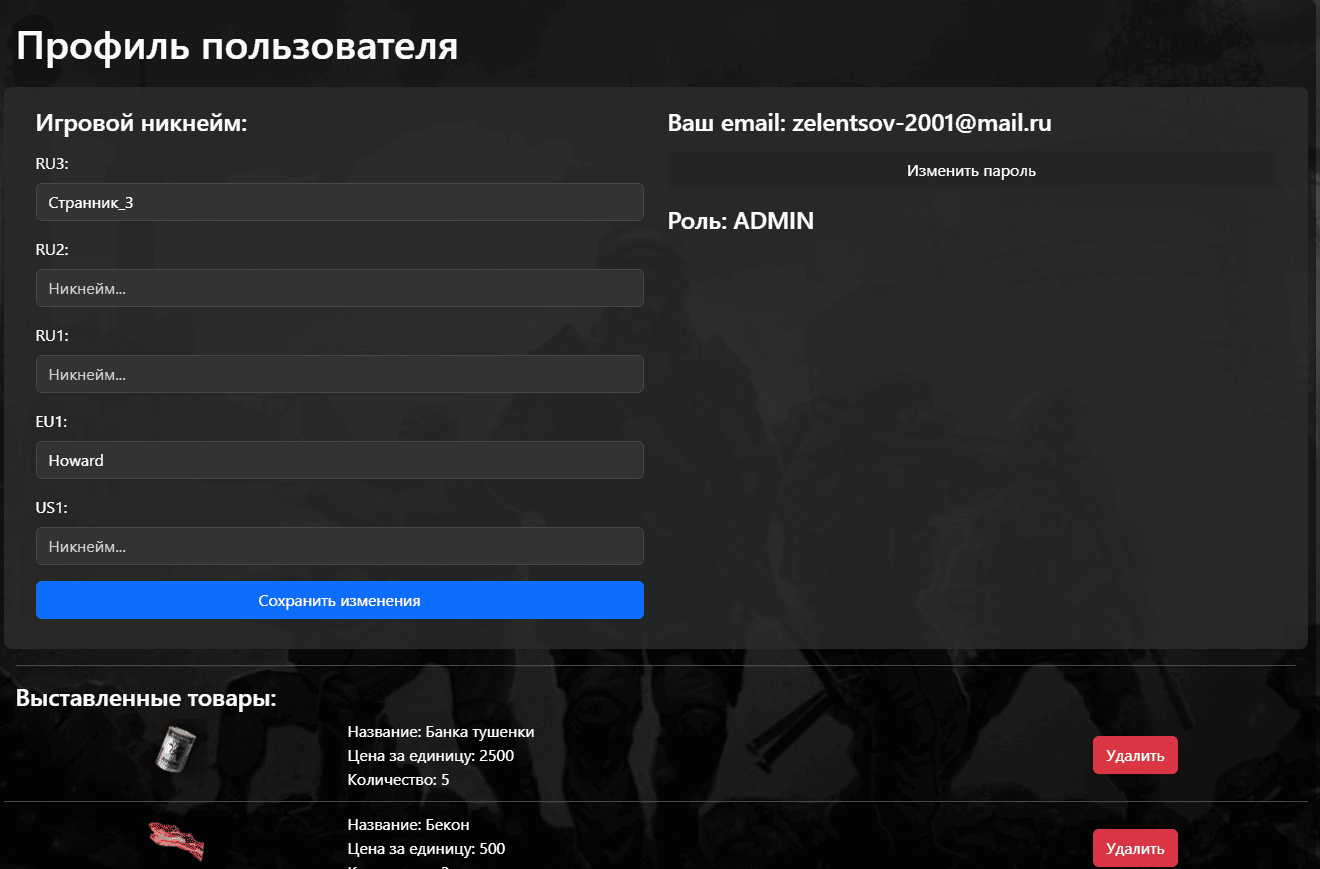
\includegraphics[width=0.7\linewidth]{images/profile_web}
	\caption{Система в состоянии «Профиль пользователя»}
	\label{fig:profileweb}
\end{figure}

После этого пользователь может поменять свой пароль на более надежный. Если введенный текущий пароль не правильный, то пользователь видит соответствующее сообщение. Если текущий пароль введен правильно, но новый пароль и повторный не совпадают, то пользователь видет соответствующее сообщение. Система в состоянии «Успешная смена пароля» представлена на рисунке \ref{fig:passwweb3}.

\begin{figure}[ht]
	\centering
	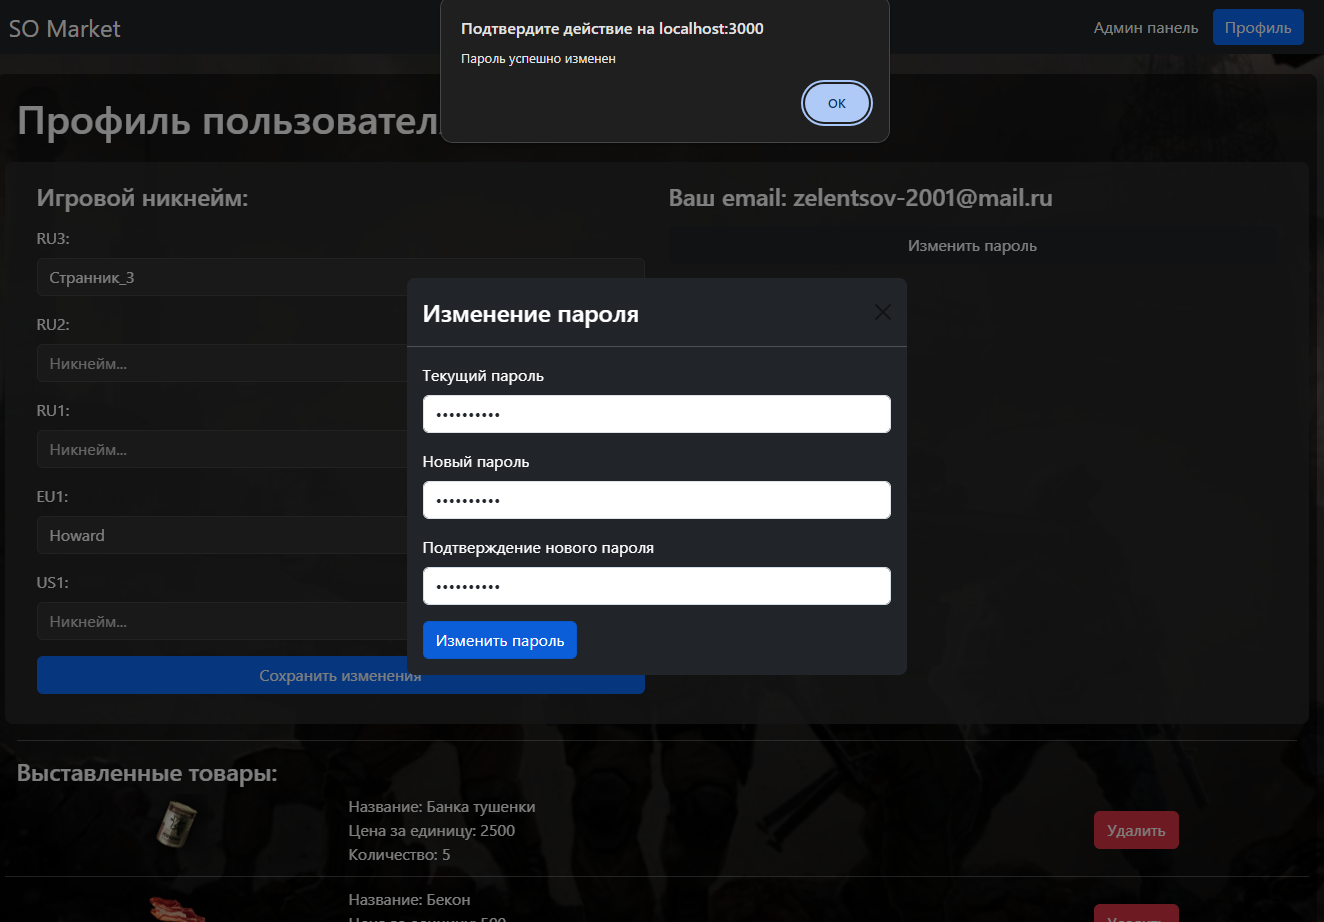
\includegraphics[width=0.7\linewidth]{images/passw_web3}
	\caption{Система в состоянии «Успешная смена пароля»}
	\label{fig:passwweb3}
\end{figure}

Система в состоянии «Неправильный текущий пароль» представлена на рисунке \ref{fig:passwweb1}.

\begin{figure}[ht]
	\centering
	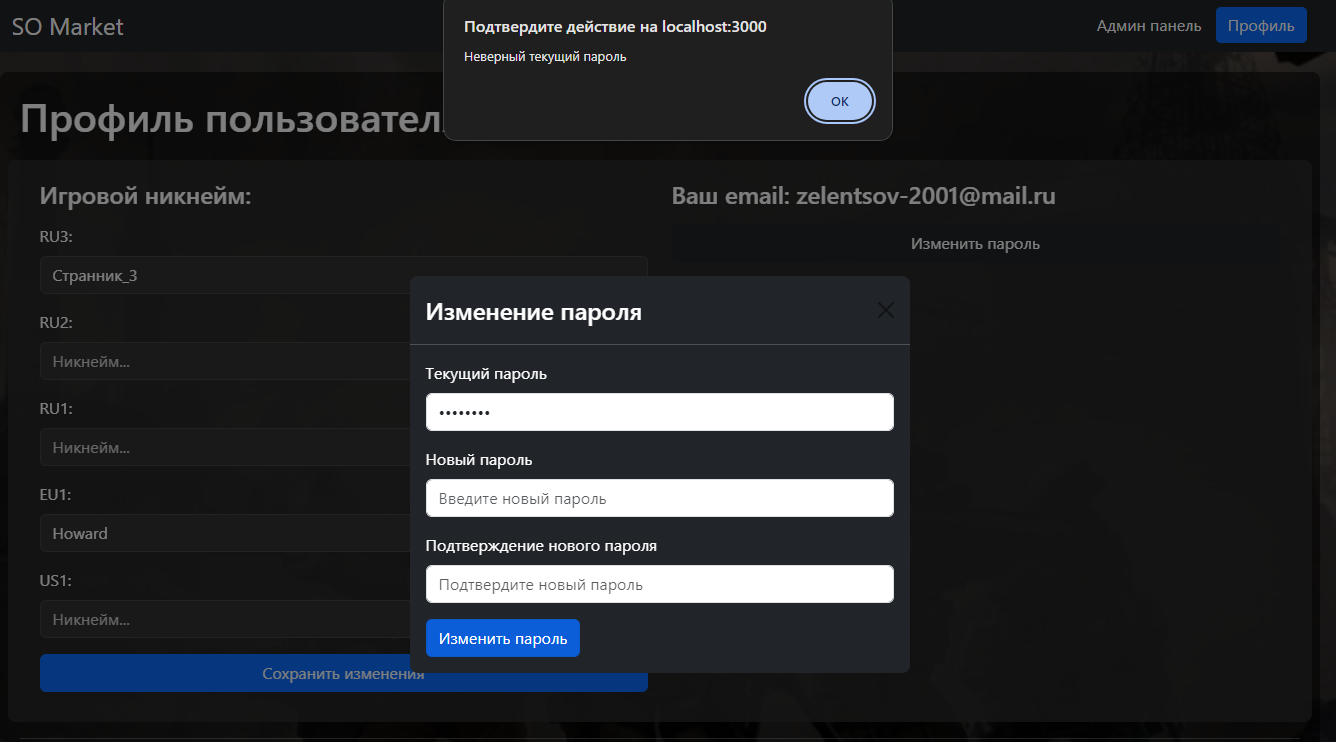
\includegraphics[width=0.7\linewidth]{images/passw_web1}
	\caption{Система в состоянии «Неправильный текущий пароль»}
	\label{fig:passwweb1}
\end{figure}

Система в состоянии «Новые пароли не совпадают» представлена на рисунке \ref{fig:passwweb2}.

\begin{figure}[ht]
	\centering
	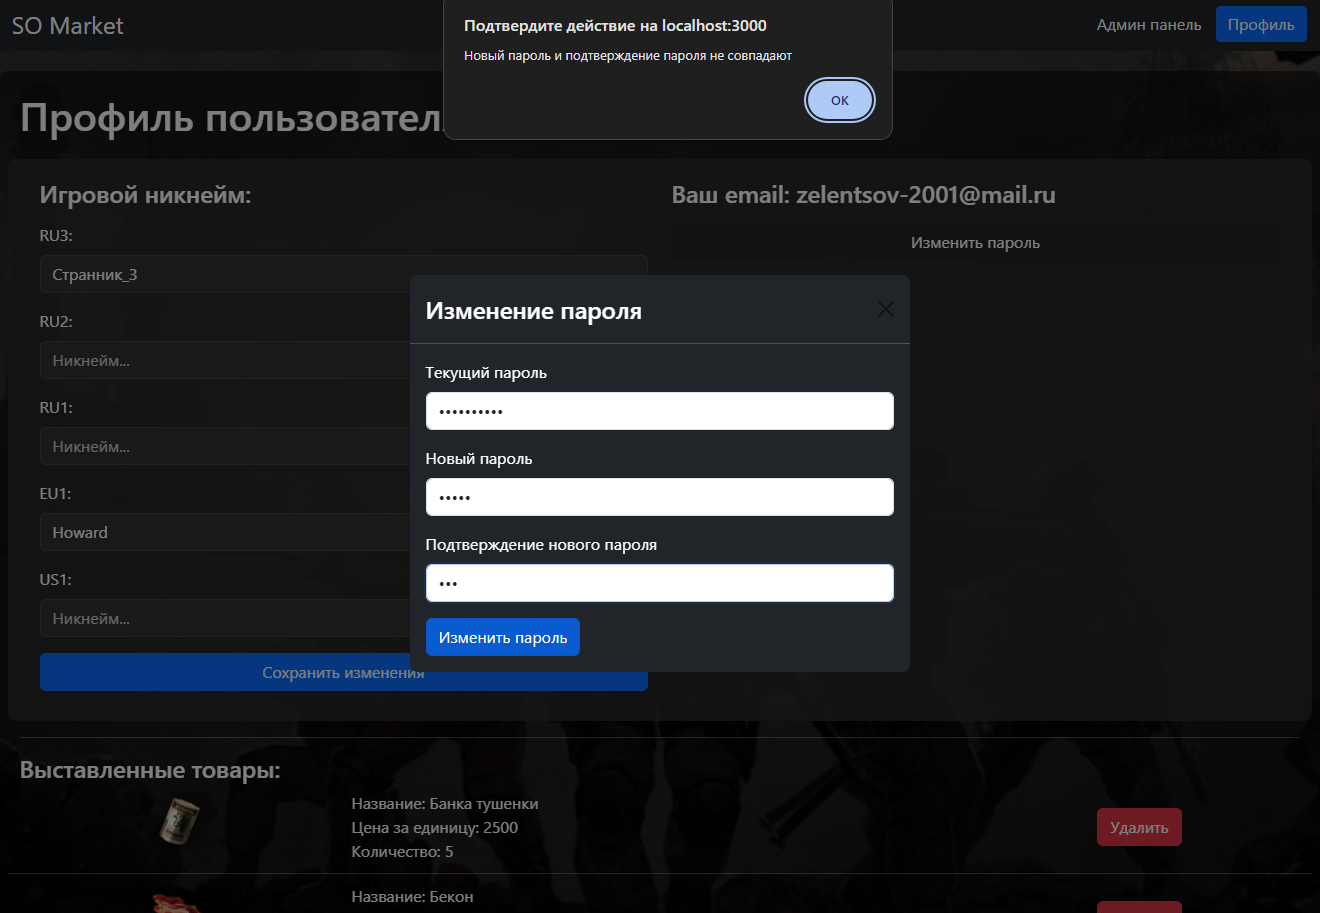
\includegraphics[width=0.7\linewidth]{images/passw_web2}
	\caption{Система в состоянии «Новые пароли не совпадают»}
	\label{fig:passwweb2}
\end{figure}

В профиле пользователь может установить свои игровые никнеймы. Система в этом состоянии представлена на рисунке \ref{fig:profilechangeweb}.

\begin{figure}[ht]
	\centering
	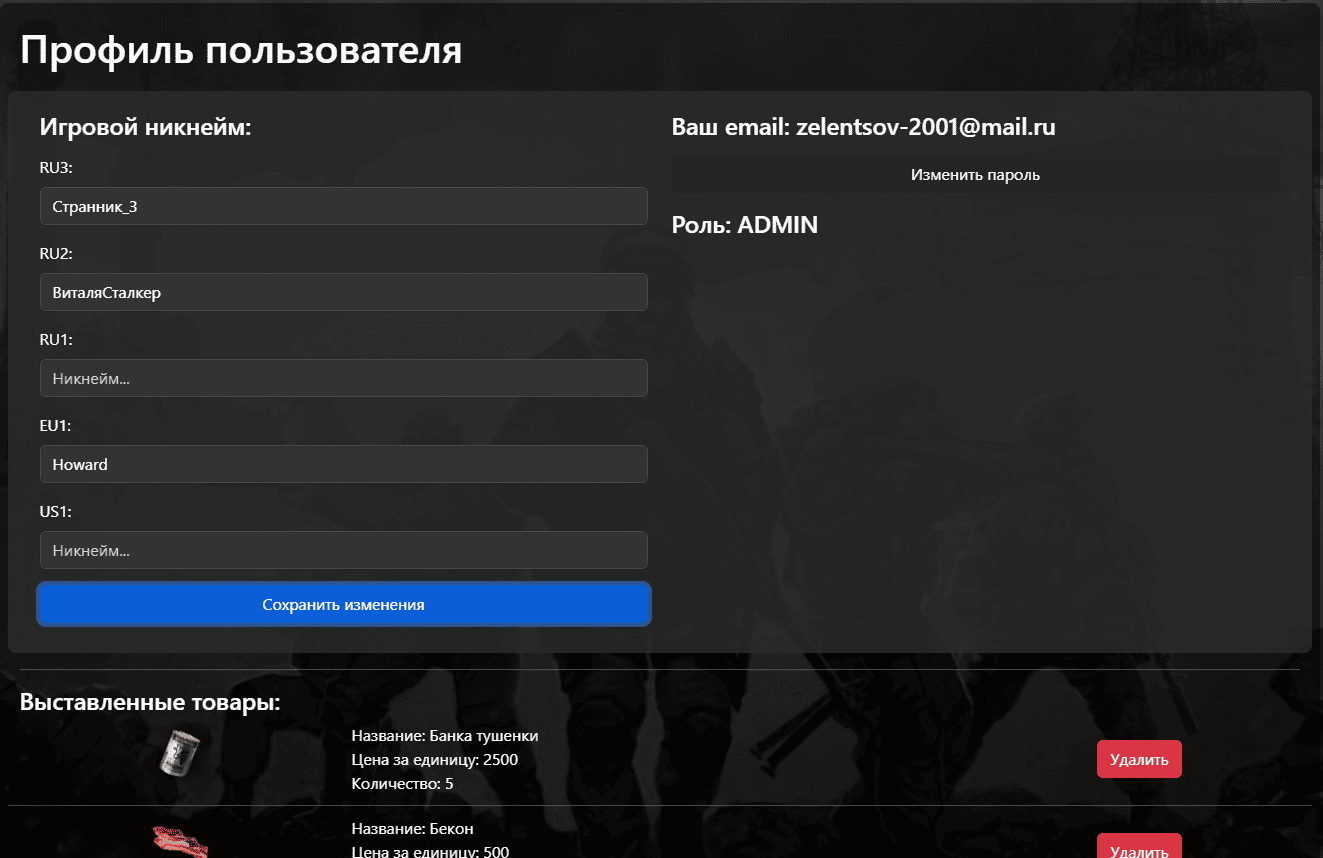
\includegraphics[width=0.7\linewidth]{images/profile_change_web}
	\caption{Система в состоянии «Сохранение никнейма»}
	\label{fig:profilechangeweb}
\end{figure}

Пользователь решил посмотреть, какие товары продают пользователи. Для этого ему необходимо выбрать интересующий его сервер. Система в этом состоянии представлена на рисунке \ref{fig:serverweb}.

\begin{figure}[ht]
	\centering
	
\includegraphics[width=0.7\linewidth]{images/server_web}
	\caption{Система в состоянии «Выбор сервера»}
	\label{fig:serverweb}
\end{figure}

После выбора сервера пользователь попадает на страницу с товарами. Система в этом состоянии представлена на рисунке \ref{fig:shopweb}.

\begin{figure}[ht]
	\centering
	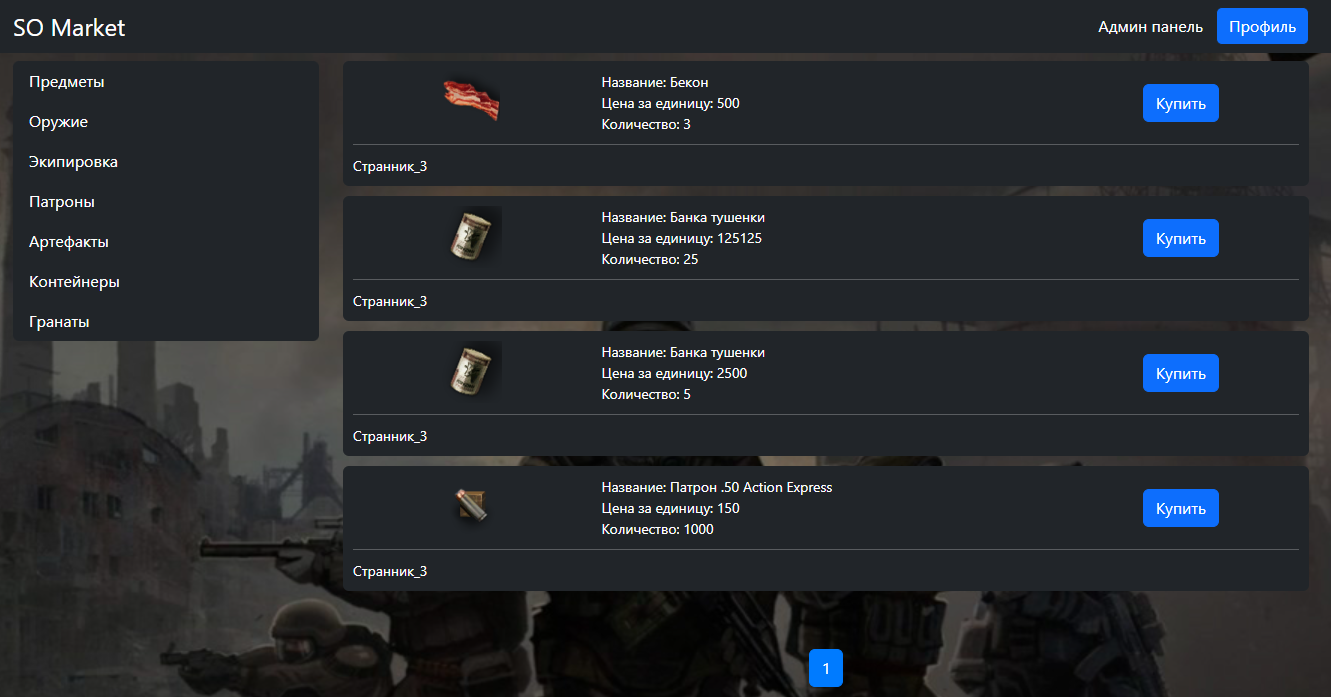
\includegraphics[width=0.7\linewidth]{images/shop_web}
	\caption{Система в состоянии «Отображение товаров»}
	\label{fig:shopweb}
\end{figure}

Пользователь может самостоятельно выбрать, какие товары отображать, установив параметры фильтрации. Система в этом состоянии представлена на рисунке \ref{fig:shopsortweb}.

\begin{figure}[ht]
	\centering
	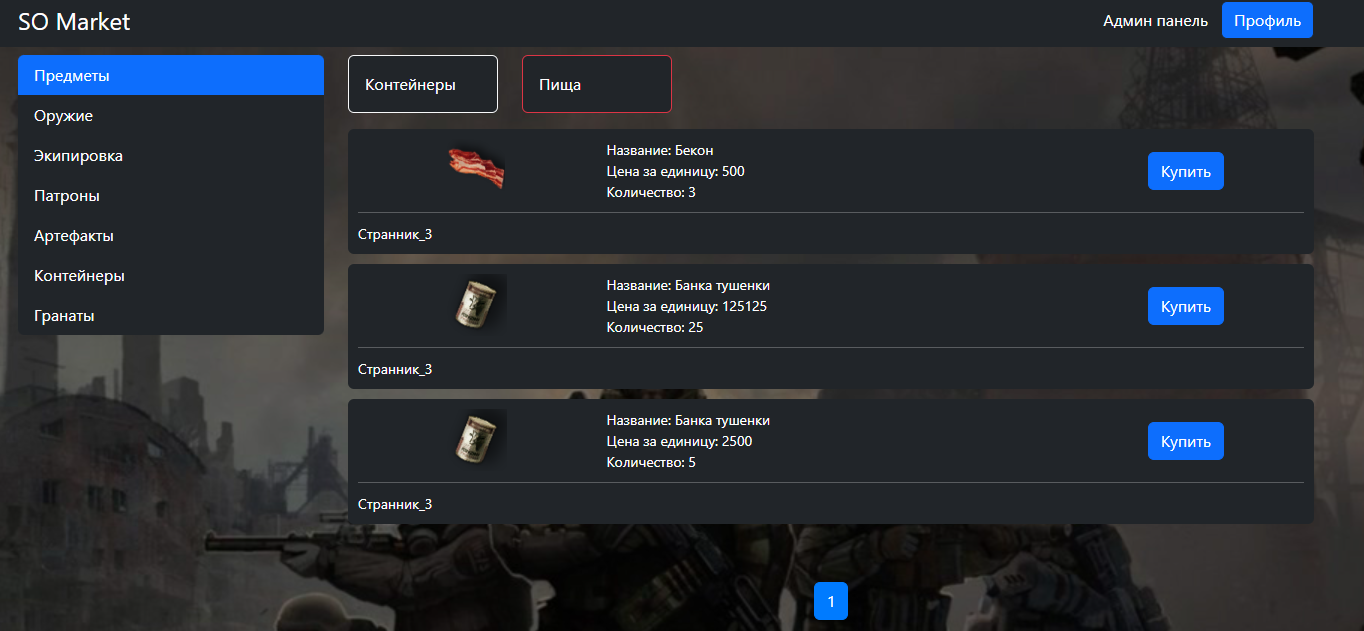
\includegraphics[width=0.7\linewidth]{images/shop_sort_web}
	\caption{Система в состоянии «Фильтрация товаров»}
	\label{fig:shopsortweb}
	
\end{figure}[ht]
Пользователь захотел сам выставить предмет на продажу. Для этого он нажимает на специальную кнопку и перед ним открывается форма. Система в состоянии «Выставить предмет на продажу» представлена на рисунке \ref{fig:sellweb}.

\begin{figure}[ht]
	\centering
	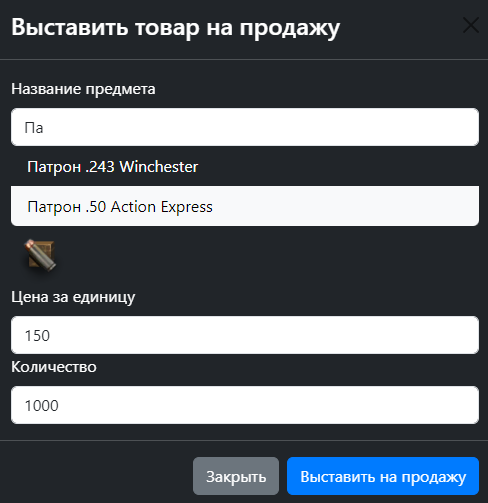
\includegraphics[width=0.6\linewidth]{images/sell_web}
	\caption{Система в состоянии «Выставить предмет на продажу»}
	\label{fig:sellweb}
	
\end{figure}[ht]
Пользователь с помощью поиска вводит название предмета, который он хочет продать и перед ним появляются все варианты, соответствующие введенным символам, вводит нужные количество предметов и их цену. Система в данном состоянии представлена на рисунке \ref{fig:sellonweb}.

\begin{figure}
	\centering
	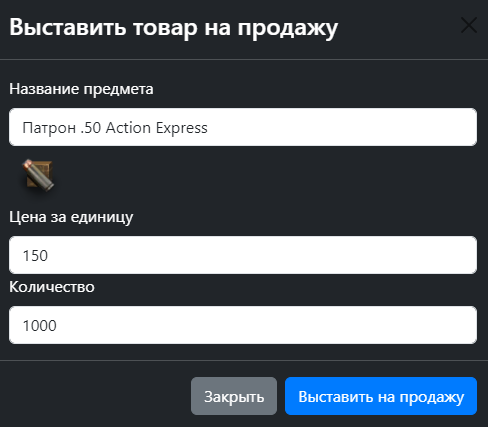
\includegraphics[width=0.7\linewidth]{images/sell_on_web}
	\caption{Система в состоянии «Продажа предмета»}
	\label{fig:sellonweb}
\end{figure}

Пользователь продал предмет или решил, что не хочет его продавать. Для этого он возвращается в профиль и нажимает на соответствующую кнопку в строке предмета. Система в этом состоянии представлена на рисунке \ref{fig:profileitemweb}.

\begin{figure}[ht]
	\centering
	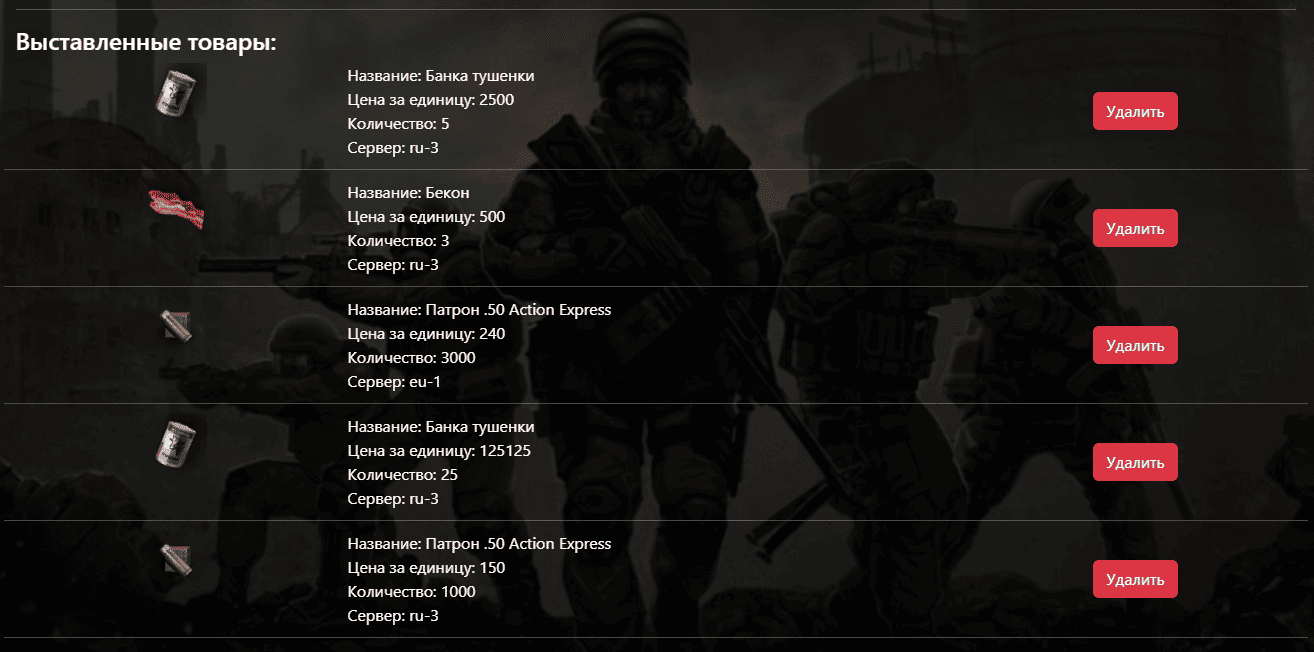
\includegraphics[width=0.7\linewidth]{images/profile_item_web}
	\caption{Система в состоянии «Отображение предметов пользователя»}
	\label{fig:profileitemweb}
\end{figure}

Пользователь решил посмотреть предметы на другом сервере. Для этого он переходит на главну юстраницу и выбирает другой сервер. Ему открывается ассортимент товаров с другого сервера. Система в данном состоянии представлена на рисунке \ref{fig:shopchangeweb}.

\begin{figure}[ht]
	\centering
	
\includegraphics[width=0.7\linewidth]{images/shop_change_web}
	\caption{Система в состоянии «Отображение товаров другого сервера»}
	\label{fig:shopchangeweb}
\end{figure}


   \section*{ЗАКЛЮЧЕНИЕ}
\addcontentsline{toc}{section}{ЗАКЛЮЧЕНИЕ}

В ходе выполнения работы была спроектирована и разработана программная система, позволяющая пользователям проще реализовывать внутриигровые ценности в игре «Stay Out». Основные результаты работы:

\begin{enumerate}
\item Проведен анализ предметной области; определены особенности предметной области и перспективы программного проекта.
\item Разработана модель данных прграммной системы; определены ключевые сущности; разработан проект базы данных.
\item Спроектированы клиентская и серверная часть программной системы; на основе требований пользователей спроектирован пользовательский интерфейс.
\item Произведено системное тестирование системы; написаны модульные тесты.
\end{enumerate}

Все требования, описанные в техническом задании, были реализованы, все задачи, поставленные в начале разработки проекта, были также решены. Дальнейшее развитие программной системы предполагает доработку и оптимизацию уже реализованных модулей, а также расширение возможностей приложения путем добавления удобной системы поиска, более компактной фильтрации, а такжедобавления состояний активности пользователя.

}\fi
\addcontentsline{toc}{section}{СПИСОК ИСПОЛЬЗОВАННЫХ ИСТОЧНИКОВ}

\begin{thebibliography}{9}

    \bibitem{javascript} Шилдт Герберт. Java полное руководство / Герберт Шилдт. – М : ООО ”И.Д. Вильяме 2015. – 1376 с. - ISBN 978-5-84-591759-1.
    \bibitem{php} Коэн Исси, Лазаро; Исси Коэн, Джозеф. Полный справочник по HTML, CSS и JavaScript / А.О. Коэн Исси, Лазаро; Исси Коэн, Джозеф. – Паблишерз : Эксмо, 2017. – 246 с. - ISBN 978-5-9790-0009-1.
    \bibitem{css} Хорстманн, К. Современный JavaScript для нетерпеливых / К. Хорстманн; перевод с английского А. А. Слинкина. — Москва: ДМК Пресс, 2021. — 288 с. — ISBN 978-5-97060-177-8.
    \bibitem{mysql}	Мандел, Т. Разработка пользовательского интерфейса / Т. Мандел. – ДМК Пресс, 2019. – 420 с. – ISBN 978-5-04-195060-6.
	\bibitem{html5}	Купер А., Рейман Р., Кронин Д., Носсел К. Интерфейс. Основы проектирования взаимодействия : [Текст] / А. Купер, Р. Рейман, Д. Кронин, К. Носсел; пер. с англ. – 4-е изд. – СПб. : Питер, 2021. – 720 с. – ISBN 978-5-4461-0877-0.
	\bibitem{htmlcss}	Джон Карнелл, Иллари Уайлупо Санчес. Микросервисы Spring в действии / пер. с англ. А. Н. Киселева. – М.: ДМК Пресс, 2022. – 490 с. - ISBN 978-5-97060-971-2.
	\bibitem{bigbook} Кугушева Дарья Сергеевна. Проектирование сложного программного обеспечения с использованием микросервисной архитектуры // Инновации и инвестиции. 2020. №5. URL: https://cyberleninka.ru/article/n/proektirovanie-slozhnogo-programmnogo-obespecheniya-s-ispolzovaniem-mikroservisnoy-arhitektury (дата обращения: 27.04.2024).
	\bibitem{uchiru} Поллард Б. HTTP/2 в действии / Б. Поллард. – Москва : ДМК Пресс, 2021. – 424 с. – ISBN 978-5-97060-925-5.
	\bibitem{chaynik}	Бауэр К., Кинг Г. Java Persistence API и Hibernate / К. Бауэр, Г. Кинг. – Москва : ДМК Пресс, 2018. – 632 с. – ISBN 978-5-97060-674-2.   
	\bibitem{22} Стойка А. Учебник по React: современное руководство / А. Стойка. – СПб: Питер, 2023. – 350 с. – ISBN 978-5-00146-705-2.    
	\bibitem{1231} Ли Дж. Руководство по React для начинающих / Дж. Ли. – М.: ДМК Пресс, 2022. – 280 с. – ISBN 978-5-97060-774-9.    
	\bibitem{sdf} Робинсон А. Express.js в действии / А. Робинсон. – М.: ДМК Пресс, 2021. – 320 с. – ISBN 978-5-97060-854-8.    
	\bibitem{servsssds} Вилсон М. Node.js для профессионалов / М. Вилсон. – СПб: Питер, 2022. – 450 с. – ISBN 978-5-00116-800-3.
	\bibitem{111} Ньюман С. Построение микросервисов / С. Ньюман. – СПб: Питер, 2020. – 360 с. – ISBN 978-5-4461-0870-1.
	\bibitem{1112} Фаулер М. Архитектура корпоративных приложений / М. Фаулер. – М.: ДМК Пресс, 2019. – 520 с. – ISBN 978-5-97060-775-6.
	\bibitem{1113} Браун Д. RESTful API Design / Д. Браун. – М.: ДМК Пресс, 2019. – 400 с. – ISBN 978-5-97060-861-6.
	\bibitem{1114} Рэмси М. Использование Axios с React.js / М. Рэмси. – М.: ДМК Пресс, 2023. – 260 с. – ISBN 978-5-97060-964-4.
	\bibitem{1115} Мессерсмит Дж. DevOps для разработки программного обеспечения / Дж. Мессерсмит. – М.: ДМК Пресс, 2021. – 370 с. – ISBN 978-5-97060-913-2.
	\bibitem{1116} Гранд Р. Полное руководство по тестированию программного обеспечения / Р. Гранд. – СПб: Питер, 2022. – 420 с. – ISBN 978-5-00117-895-8.
	\bibitem{1117} Фриман Э. Архитектура программного обеспечения / Э. Фриман. – М.: ДМК Пресс, 2021. – 480 с. – ISBN 978-5-97060-973-6.
	\bibitem{1118} Мартин Р. Чистый код: создание, анализ и рефакторинг / Р. Мартин. – М.: Питер, 2020. – 464 с. – ISBN 978-5-496-00667-5.
\end{thebibliography}

\ifВКР{\appendix{Представление графического материала}

Графический материал, выполненный на отдельных листах,
изображен на рисунках А.1--А.\arabic{числоПлакатов}.
\setcounter{числоПлакатов}{0}

\renewcommand{\thefigure}{А.\arabic{figure}} % шаблон номера для плакатов

\begin{landscape}

\begin{плакат}
    \includegraphics[width=0.82\linewidth]{плакат1.png}
    \заголовок{Сведения о ВКРБ}
    \label{pl1:image}      
\end{плакат}

\begin{плакат}
    \includegraphics[width=0.82\linewidth]{плакат2.png}
    \заголовок{Цели и задачи разработки}
    \label{pl2:image}      
\end{плакат}

\begin{плакат}
    \includegraphics[width=0.82\linewidth]{плакат3.png}
    \заголовок{Концептуальная диаграмма сущность-связь}
    \label{pl3:image}      
\end{плакат}

\begin{плакат}
    \includegraphics[width=0.82\linewidth]{плакат4.png}
    \заголовок{Диаграмма прецедентов}
    \label{pl4:image}      
\end{плакат}

\begin{плакат}
	\centering
	\includegraphics[width=0.82\linewidth]{images/плакат5}
	\caption{Диаграмма компонентов}
	\label{pl5:image}
\end{плакат}

\begin{плакат}
	\centering
	\includegraphics[width=0.82\linewidth]{images/плакат6}
	\caption{Диаграмма размещения}
	\label{pl6:image}
\end{плакат}

\begin{плакат}
	\centering
	\includegraphics[width=0.82\linewidth]{images/плакат7}
	\caption{Карта маршрутов}
	\label{pl7:image}
\end{плакат}


\end{landscape}
}\fi
\ifПрактика{}\else{\appendix{Фрагменты исходного кода программы}
ClassController.js
\begin{lstlisting}[language=C++]
	const { Class } = require("../models/models")
	
	class ClassController {
		
		async create(req, res) {
			try {
				let {name, typeId} = req.body
				const clas = await Class.create({name, typeId})
				return res.json(clas)
			} catch (error) {
				console.error("Error creating class:", error);
				return res.status(500).json({ message: "Internal server error" });
			}
		}
		
		async getAll(req, res) {
			const clases = await Class.findAll()
			return res.json(clases)
		}
	}
	
	module.exports = new ClassController()
\end{lstlisting}

itemController.js
\begin{lstlisting}[language=C++]
	const uuid = require('uuid')
	const path = require('path')
	const {Item, AmmoInfo, Equipment, Weapon, Containers, Artefacts, Grenades, StorageItem, User, Type, Class} = require('../models/models')
	const ApiError = require('../error/ApiError')
	const { Op } = require('sequelize')
	
	class ItemController {
		
		async create(req, res, next) {
			try {
				let {name, description, weight, level, typeId, classId, ammo_infos, artefacts, equipment, weapons, containers, grenade} = req.body
				const {img} = req.files
				let fileName = uuid.v4() + ".png"
				img.mv(path.resolve(__dirname, '..', 'static', fileName))
				
				const item = await Item.create({name, description, weight, level, typeId, classId, img: fileName})
				
				if (ammo_infos) {
					ammo_infos = JSON.parse(ammo_infos);
					ammo_infos.forEach(async i => {
						await AmmoInfo.create({
							type_ammo: i.type_ammo,
							breaking_throught: i.breaking_throught,
							damage: i.damage,
							itemId: item.id
						});
					});
				}
				
				if (weapons) {
					weapons = JSON.parse(weapons);
					weapons.forEach(async i => {
						await Weapon.create({
							moa: i.moa, 
							rate_of_fire: i.rate_of_fire, 
							breaking_throught: i.breaking_throught, 
							strength: i.strength, 
							recoil: i.recoil,
							handing: i.handing,
							state_waivers: i.state_waivers,
							nopollution: i.nopollution,
							itemId: item.id
						})
					})
				}
				
				return res.json(item)
			} catch (e) {
				next(ApiError.badRequest(e.message))
			}
		}
		
		async getAll(req, res) {
			let {classId, typeId, limit, page} = req.query
			page = page || 1
			limit = limit || 15
			let offset = page * limit - limit
			let items;
			if (!classId && !typeId) {
				items = await Item.findAndCountAll({limit, offset})
			}
			if (classId && !typeId) {
				items = await Item.findAndCountAll({where:{classId}, limit, offset})
			}
			if(!classId && typeId) {
				items = await Item.findAndCountAll({where:{typeId}, limit, offset})
			}
			if (classId && typeId) {
				items = await Item.findAndCountAll({where:{classId, typeId}, limit, offset})
			}
			return res.json(items)
		}
		
		async getOne(req, res) {
			const {id} = req.params
			const item = await Item.findOne(
			{
				where: {id},
				include: [{model: AmmoInfo, as: 'ammo_infos'}]
			}
			)
			return res.json(item)
		}
		
		async search(req, res) {
			const { name } = req.params;
			
			if (!name) {
				return res.status(400).json({ message: 'Название предмета не может быть пустым' });
			}
			
			try {
				const items = await Item.findAll({
					where: {
						name: {
							[Op.like]: `%${name}%`
						}
					}
				});
				return res.json(items);
			} catch (error) {
				console.error('Ошибка при поиске предмета:', error);
				return res.status(500).json({ message: 'Ошибка при поиске предмета' });
			}
		}
		
		async getStorageItems(req, res, next) {
			const { server } = req.params
			let { page, limit, classId, typeId } = req.query;
			page = page || 1
			limit = limit || 15
			let offset = page * limit - limit
			
			const where = {};
			if (classId) where.classId = classId;
			if (typeId) where.typeId = typeId;
			
			try {
				const items = await StorageItem.findAndCountAll({
					where: { server },
					include: [
					{
						model: Item,
						attributes: ['id', 'name', 'img']
					},
					{
						model: User,
						attributes: ['id', 'email', 'ru1', 'ru2', 'ru3', 'eu1', 'us1']
					}
					],
					limit,
					offset,
					order: [
					['itemId', 'ASC'],
					['userId', 'ASC']
					]
				});
				
				return res.json(items);
			} catch (error) {
				console.error("Ошибка при получении предметов из хранилища:", error); // Логируем ошибку
				next(ApiError.internal(error.message));
			}
		}
		
		async getUserItems(req, res, next) {
			const { userId } = req.query;
			
			try {
				const items = await StorageItem.findAll({
					where: { userId },
					include: [
					{
						model: Item,
						attributes: ['id', 'name', 'img']
					},
					{
						model: User,
						attributes: ['id', 'email']
					}
					],
					order: [['id', 'ASC']]
				});
				
				return res.json(items);
			} catch (error) {
				console.error("Ошибка при получении предметов пользователя:", error);
				next(ApiError.internal(error.message));
			}
		}
		
		async addItemToStorage(req, res, next) {
			const { userId, itemId, price, quantity, classId, typeId, server } = req.body;
			try {
				// Создаем запись в StorageItem
				const storageItem = await StorageItem.create({
					userId,
					itemId,
					price,
					quantity,
					classId,
					typeId,
					server
				});
				
				return res.json(storageItem);
			} catch (error) {
				return next(error);
			}
		}
		
		async deleteItem(req, res, next) {
			try {
				const { id } = req.params;
				const item = await StorageItem.findOne({ where: { id } });
				
				if (!item) {
					return next(ApiError.badRequest('Предмет не найден'));
				}
				
				// Удаление предмета из базы данных
				await item.destroy();
				
				return res.json({ message: 'Предмет успешно удален' });
			} catch (error) {
				console.error('Ошибка при удалении предмета:', error);
				next(ApiError.internal('Ошибка при удалении предмета'));
			}
		}
		
		async getAmmoInfosByItemId(req, res, next) {
			const { itemId } = req.params;
			try {
				const ammoInfos = await AmmoInfo.findAll({ where: { itemId } });
				return res.json(ammoInfos);
			} catch (error) {
				console.error('Error fetching ammo_infos:', error);
				return res.status(500).json({ error: 'Internal server error' });
			}
		}
	}
	
	module.exports = new ItemController()
\end{lstlisting}
	
typeController.js
\begin{lstlisting}[language=C++]
	const {Type} = require('../models/models');
	const ApiError = require('../error/ApiError');
	
	class TypeController {
		
		async create(req, res) {
			const {name} = req.body
			const type = await Type.create({name})
			return res.json(type)
		}
		
		async getAll(req, res) {
			const types = await Type.findAll()
			return res.json(types)
		}
	}
	
	module.exports = new TypeController()
\end{lstlisting}

userController.js
\begin{lstlisting}[language=C++]
	const ApiError = require('../error/ApiError');
	const bcrypt = require('bcrypt')
	const jwt = require('jsonwebtoken')
	const {User, Storage, StorageItem, Item} = require('../models/models')
	
	const generateJwt = (id, email, role, ru1, ru2, ru3, eu1, us1) => {
		return jwt.sign(
		{id: id, email, role, ru1, ru2, ru3, eu1, us1}, 
		process.env.SECRET_KEY,
		{expiresIn: '24h'}
		)
	}
	
	class UserController {
		
		async registration(req, res, next) {
			const {email, password, role} = req.body
			if (!email || !password) {
				return next(ApiError.badRequest('Некорректный email или password'))
			}
			const candidate = await User.findOne({where: {email}})
			if (candidate) {
				return next(ApiError.badRequest('Пользователь с таким email уже существует'))
			}
			const hashPassword = await bcrypt.hash(password, 5)
			const user = await User.create({email, role, password: hashPassword})
			const basket = await Storage.create({userId: user.id})
			const token = generateJwt(user.id, user.email, user.role, user.ru1, user.ru2, user.ru3, user.eu1, user.us1)
			return res.json({token})
		}
		
		async login(req, res, next) {
			const {email, password} = req.body
			const user = await User.findOne({where: {email}})
			if (!user) {
				return next(ApiError.internal('Пользователь с таким именем не найден'))
			}
			let comparePassword = bcrypt.compareSync(password, user.password)
			if (!comparePassword) {
				return next(ApiError.internal('Указан неверный пароль'))
			}
			const token = generateJwt(user.id, user.email, user.role, user.ru1, user.ru2, user.ru3, user.eu1, user.us1)
			return res.json({token})
		}
		
		async check(req, res, next) {
			const token = generateJwt(req.user.id, req.user.email, req.user.role, req.user.ru1, req.user.ru2, req.user.ru3, req.user.eu1, req.user.us1)
			return res.json({token})
		}
		
		async changePassword(req, res, next) {
			const { currentPassword, newPassword } = req.body;
			const userId = req.user.id;
			
			const user = await User.findOne({ where: { id: userId } });
			if (!user) {
				return next(ApiError.badRequest('Пользователь не найден'));
			}
			
			const isPasswordValid = await bcrypt.compare(currentPassword, user.password);
			if (!isPasswordValid) {
				return next(ApiError.badRequest('Неверный текущий пароль'));
			}
			
			const hashPassword = await bcrypt.hash(newPassword, 5);
			user.password = hashPassword;
			await user.save();
			
			return res.json({ message: 'Пароль успешно изменен' });
		}
		
		async createStorage(req, res, next) {
			const { userId } = req.body;
			const storage = await Storage.create({ userId });
			return res.json(storage);
		}
		
		async addItemToStorage(req, res, next) {
			const { storageId, itemId, price, quantity } = req.body;
			const storageItem = await StorageItem.create({ storageId, itemId, price, quantity });
			return res.json(storageItem);
		}
		
		async getItemsFromStorage(req, res, next) {
			const { storageId, classId, typeId, limit, page } = req.query;
			const items = await StorageItem.findAll({
				where: { storageId },
				include: [
				{
					model: Item,
					where: {
						...(classId && { classId }),
						...(typeId && { typeId })
					}
				}
				],
				limit,
				offset: (page - 1) * limit
			});
			return res.json(items);
		}
		
		async updateNicknames(req, res, next) {
			const { userId, nicknames } = req.body;
			
			// Логирование входящих данных
			console.log("updateNicknames - userId:", userId);
			console.log("updateNicknames - nicknames:", nicknames);
			
			if (!userId) {
				return next(ApiError.badRequest('User ID is required'));
			}
			
			try {
				const user = await User.findByPk(userId);
				
				if (!user) {
					return next(ApiError.notFound('User not found'));
				}
				
				user.ru3 = nicknames.ru3 || user.ru3;
				user.ru2 = nicknames.ru2 || user.ru2;
				user.ru1 = nicknames.ru1 || user.ru1;
				user.eu1 = nicknames.eu1 || user.eu1;
				user.us1 = nicknames.us1 || user.us1;
				
				await user.save();
				
				return res.json({ message: 'Nicknames updated successfully' });
			} catch (error) {
				console.error('Error updating nicknames:', error);
				return next(ApiError.internal(error.message));
			}
		}
	}
	
	module.exports = new UserController()
\end{lstlisting}

Main.js
\begin{lstlisting}[language=C++]
	import React, { useState } from "react";
	import { Button, Container } from "react-bootstrap";
	import ServerSelectModal from "../components/ServerSelectModal";
	
	const Main = () => {
		const [modalShow, setModalShow] = useState(false)
		return (
		<div className="home-background">
		<Container className="text-center text-white d-flex flex-column justify-content-center align-items-center vh-100">
		<h1>SO MARKET</h1>
		<h2>УДОБНАЯ ПЛОЩАДКА ДЛЯ ТОРГОВЛИ</h2>
		<p>Для начала выберите свой сервер</p>
		<Button variant="outline-light" className="mt-3" onClick={() => setModalShow(true)}>Выбрать сервер</Button>
		
		<ServerSelectModal show={modalShow} handleClose={() => setModalShow(false)} />
		</Container>
		</div>
		);
	};
	
	export default Main;
\end{lstlisting}

ProfilPage.js
\begin{lstlisting}[language=C++]
	import React, { useContext, useState, useEffect } from 'react';
	import { Container, Row, Col, Button, Form, Image } from 'react-bootstrap';
	import './ProfilPage.css';
	import ChangePasswordModal from "../components/modals/ChangePasswordModal";
	import { Context } from '../index';
	import { check, updateNickname } from '../http/userAPI';
	import { deleteUserItem, fetchUserItems } from '../http/ItemAPI';
	import { useNavigate } from 'react-router-dom';
	import { DEVICE_ROUTE } from '../utils/consts';
	
	const Profile = () => {
		const { user } = useContext(Context);
		const [showChangePasswordModal, setShowChangePasswordModal] = useState(false);
		const [nicknames, setNicknames] = useState({
			ru3: '',
			ru2: '',
			ru1: '',
			eu1: '',
			us1: ''
		});
		const [items, setItems] = useState([]);
		const [userData, setUserData] = useState({ id: 0, email: '', role: '' });
		const navigate = useNavigate();
		
		useEffect(() => {
			const fetchData = async () => {
				try {
					const user = await check();
					
					if (user) {
						const { userId, email, role } = user;
						setUserData({ id: userId, email, role });
						
						console.log("Fetched user data:", user);
						
						// Получение предметов пользователя после установки userData
						const userItems = await fetchUserItems(userId);
						setItems(userItems);
						
						setNicknames({
							ru3: user.ru3 || '',
							ru2: user.ru2 || '',
							ru1: user.ru1 || '',
							eu1: user.eu1 || '',
							us1: user.us1 || ''
						});
					} else {
						console.error('Ошибка аутентификации пользователя');
					}
				} catch (error) {
					console.error('Ошибка при загрузке данных пользователя:', error);
				}
			};
			
			fetchData();
		}, []);
		
		const handleOpenChangePasswordModal = () => setShowChangePasswordModal(true);
		const handleCloseChangePasswordModal = () => setShowChangePasswordModal(false);
		
		const handleInputChange = (event) => {
			const { id, value } = event.target;
			setNicknames((prevState) => ({
				...prevState,
				[id]: value
			}));
		};
		
		const handleSaveNicknames = async () => {
			try {
				await updateNickname(userData.id, nicknames);
			} catch (error) {
				console.error('Ошибка при сохранении никнеймов:', error);
			}
		};
		
		const handleDeleteItem = async (itemId) => {
			try {
				await deleteUserItem(itemId);
				setItems(items.filter(item => item.id !== itemId));
			} catch (error) {
				console.error('Ошибка при удалении предмета:', error);
			}
		};
		
		return (
		<>
		<div className="profile-background"></div>
		<Container className="profile-container">
		<h1 className="profile-title">Профиль пользователя</h1>
		<Row className="profile-row">
		<Col md={6}>
		<h4>Игровой никнейм:</h4>
		<Form>
		{Object.keys(nicknames).map((key) => (
			<Form.Group className="mb-3" controlId={key} key={key}>
			<Form.Label>{key.toUpperCase().replace('_', '-')}:</Form.Label>
			<Form.Control 
			type="text" 
			placeholder="Никнейм..." 
			value={nicknames[key]} 
			onChange={handleInputChange} 
			/>
			</Form.Group>
			))}
		<Button variant="primary" onClick={handleSaveNicknames}>Сохранить изменения</Button>
		</Form>
		</Col>
		<Col md={6}>
		<h4>Ваш email: {userData.email}</h4>
		<Button variant="dark" className="mb-3" onClick={handleOpenChangePasswordModal}>Изменить пароль</Button>
		<h4>Роль: {userData.role}</h4>
		</Col>
		</Row>
		<hr />
		<Row>
		<h4>Выставленные товары:</h4>
		{items.map(item => (
			<React.Fragment key={item.id}>
			<Row className="h-100" style={{ marginRight: 0, marginLeft: 0 }}>
			<Col md={3} className="h-100 d-flex align-items-center justify-content-center" style={{ paddingRight: 0, paddingLeft: 0 }}>
			<Image
			src={process.env.REACT_APP_API_URL + item.item.img}
			fluid
			style={{ maxHeight: '100%', width: 'auto' }}
			onClick={() => navigate(DEVICE_ROUTE + '/' + item.id)}
			/>
			</Col>
			<Col md={6} className="d-flex align-items-center">
			<div>
			<div>{"Название: " + item.item.name}</div>
			<div>{"Цена за единицу: " + item.price}</div>
			<div>{"Количество: " + item.quantity}</div>
			<div>{"Сервер: " + item.server}</div>
			</div>
			</Col>
			<Col md={3} className="d-flex align-items-center justify-content-center">
			<Button variant="danger" onClick={() => handleDeleteItem(item.id)}>Удалить</Button>
			</Col>
			</Row>
			<hr style={{ margin: '10px 0' }} />
			</React.Fragment>
			))}
		</Row>
		<ChangePasswordModal
		show={showChangePasswordModal}
		handleClose={handleCloseChangePasswordModal}
		/>
		</Container>
		</>
		);
	};
	
	export default Profile;
\end{lstlisting}

Shop.js
\begin{lstlisting}[language=C++]
	import React, { useContext, useEffect, useState } from "react";
	import { Button, Col, Container, Form, ListGroup, Row } from "react-bootstrap";
	import TypeBar from "../components/TypeBar";
	import ClassBar from "../components/ClassBar";
	import ItemList from "../components/ItemList";
	import { observer } from "mobx-react-lite";
	import { Context } from "../index";
	import { fetchClasses, fetchItem, fetchStorageItems, fetchTypes, searchItemByName } from "../http/ItemAPI";
	import Pages from "../components/Pages";
	import '../App.css';
	import SellItemModal from "../components/modals/SellItemModal";
	import { useNavigate, useParams } from "react-router-dom";
	
	const Shop = observer(() => {
		const {user, device} = useContext(Context);
		const navigate = useNavigate();
		const { serverId } = useParams();
		const [showModal, setShowModal] = useState(false);
		
		const handleSellItem = async () => {
			setShowModal(false);
		};
		
		useEffect(() => {
			const fetchData = async () => {
				try {
					const typesData = await fetchTypes();
					device.setTypes(typesData);
					
					const classesData = await fetchClasses();
					device.setClasses(classesData);
					
					const storageItemsData = await fetchStorageItems(serverId, device.selectedType.id, device.selectedClass.id, device.page, 5);
					device.setItems(storageItemsData.rows);
					device.setTotalCount(storageItemsData.count);
				} catch (error) {
					console.error('Ошибка при загрузке данных:', error);
				}
			};
			
			fetchData();
			
			const intervalId = setInterval(fetchData, 5000);
			
			return () => clearInterval(intervalId);
		}, [device.selectedType, device.selectedClass, device.page, serverId]);
		
		return (
		<Container>
		<Row className="mt-2">
		<Col md={3}>
		<TypeBar />
		</Col>
		<Col md={9}>
		<ClassBar />
		<ItemList serverId={serverId} />
		<Pages />
		</Col>
		</Row>
		<Button variant="primary" onClick={() => setShowModal(true)} style={{ position: 'fixed', bottom: '20px', right: '20px' }}>
		<i className="fas fa-plus"></i> Выставить на продажу
		</Button>
		<SellItemModal show={showModal} handleClose={() => setShowModal(false)} handleSell={handleSellItem} serverId={serverId} />
		</Container>
		);
	});
	
	export default Shop;
\end{lstlisting}

Auth.js
\begin{lstlisting}[language=C++]
	import React, { useContext, useState } from "react";
	import { Button, Card, Col, Container, Row } from "react-bootstrap";
	import { Form } from "react-bootstrap";
	import { NavLink, useLocation, useNavigate } from "react-router-dom";
	import { LOGIN_ROUTE, MAIN_ROUTE, REGISTRATION_ROUTE } from "../utils/consts";
	import { login, registration } from "../http/userAPI";
	import { observer } from "mobx-react-lite";
	import { Context } from "../index";
	
	const Auth = observer(() => {
		const {user} = useContext(Context)
		const location = useLocation()
		const history = useNavigate()
		const isLogin = location.pathname === LOGIN_ROUTE
		const [email, setEmail] = useState('')
		const [password, setPassword] = useState('')
		
		const click = async () => {
			try {
				let data;
				if (isLogin) {
					data = await login(email, password)
				} else {
					data = await registration(email, password)
				}
				user.setUser(user)
				user.setIsAuth(true)
				history(MAIN_ROUTE)
			} catch(e) {
				alert(e.response.data.message)
			}
		}
		
		return (
		<Container 
		className="d-flex justify-content-center align-items-center"
		style={{height: window.innerHeight - 54}}
		>
		<Card style={{width: 600}} className="p-5">
		<h2 className="m-auto">{isLogin ? "Авторизация" : "Регистрация"}</h2>
		<Form className="d-flex flex-column">
		<Form.Control
		className="mt-4"
		placeholder="Введите ваш email..."
		value={email}
		onChange={e => setEmail(e.target.value)}
		/>
		<Form.Control
		className="mt-3"
		placeholder="Введите ваш пароль..."
		value={password}
		onChange={e => setPassword(e.target.value)}
		type="password"
		/>
		<Row className="d-flex justify-content-between align-items-center mt-3">
		{isLogin ? 
			<Col className="pl-0">
			Нет аккаунта? <NavLink to={REGISTRATION_ROUTE}>Зарегистрируйтесь!</NavLink>
			</Col>
			:
			<Col className="pl-0">
			Есть аккаунт? <NavLink to={LOGIN_ROUTE}>Войдите!</NavLink>
			</Col>
		}
		{isLogin ? 
			<Col className="d-flex justify-content-end pr-0">
			<Button variant="outline-success" onClick={click}>Войти</Button>
			</Col>
			:
			<Col className="d-flex justify-content-end pr-0">
			<Button variant="outline-success" onClick={click}>Зарегистрироваться</Button>
			</Col>
		}
		</Row>
		</Form>
		</Card>
		</Container>
		);
	});
	
	export default Auth;
\end{lstlisting}

ItemItem.js
\begin{lstlisting}[language=C++]
	import React, { useState } from 'react';
	import { Card, Col, Image, Button, Row, Form } from 'react-bootstrap';
	import { useNavigate } from 'react-router-dom';
	import { DEVICE_ROUTE } from '../utils/consts';
	
	const ItemItem = ({ device, serverId }) => {
		const navigate = useNavigate();
		const [isBuying, setIsBuying] = useState(false);
		const formattedServerId = serverId.serverId.replace('-', '');
		
		const userNickname = device.user[formattedServerId];
		
		const handleBuyClick = () => {
			setIsBuying(true);
		};
		
		const handleCancelClick = () => {
			setIsBuying(false);
		};
		
		return (
		<Col md={12}>
		<Card id='cardItem' style={{ cursor: 'pointer', marginBottom: '10px', padding: '10px', fontSize: '14px' }} border="light">
		{!isBuying ? (
			<>
			<Row className="h-100" style={{ marginRight: 0, marginLeft: 0 }}>
			<Col md={3} className="h-100 d-flex align-items-center justify-content-center" style={{ paddingRight: 0, paddingLeft: 0 }}>
			<Image
			src={process.env.REACT_APP_API_URL + device.item.img}
			fluid
			style={{ maxHeight: '100%', width: 'auto' }}
			onClick={() => navigate(DEVICE_ROUTE + '/' + device.item.id)}
			/>
			</Col>
			<Col md={6} className="d-flex align-items-center">
			<div>
			<div>{"Название: " + device.item.name}</div>
			<div>{"Цена за единицу: " + device.price}</div>
			<div>{"Количество: " + device.quantity}</div>
			</div>
			</Col>
			<Col md={3} className="d-flex align-items-center justify-content-center">
			<Button variant="primary" onClick={handleBuyClick}>Купить</Button>
			</Col>
			</Row>
			<hr style={{ margin: '10px 0' }} />
			<Row className="d-flex justify-content-center">
			<div>{"  " + userNickname}</div>
			</Row>
			</>
			) : (
			<>
			<Row className="h-100" style={{ marginRight: 0, marginLeft: 0 }}>
			<Col md={12}>
			<div style={{ marginBottom: '5px' }}>Скопируйте сообщение ниже:</div>
			<Form.Control
			as="textarea"
			rows={3}
			defaultValue={`@${userNickname} Привет. Хочу купить: "${device.item.name}" за ${device.price} рублей (somarket)`}
			style={{ fontSize: '14px' }}
			/>
			</Col>
			</Row>
			<hr style={{ margin: '10px 0' }} />
			<Row className="d-flex justify-content-center">
			<Button variant="outline-danger" size="sm" onClick={handleCancelClick} style={{ width: 'auto', margin: '5 auto' }}>Закрыть</Button>
			</Row>
			</>
			)}
		</Card>
		</Col>
		);
	};
	
	export default ItemItem;
\end{lstlisting}

itemAPI.js
\begin{lstlisting}[language=C++]
	import { $authHost, $host } from "./index";
	
	export const createType = async (type) => {
		const {data} = await $authHost.post('api/type', type);
		return data;
	};
	
	export const fetchTypes = async () => {
		const {data} = await $host.get('api/type');
		return data;
	};
	
	export const createClass = async (classe) => {
		const {data} = await $authHost.post('api/class', classe);
		return data;
	};
	
	export const fetchClasses = async () => {
		const {data} = await $host.get('api/class');
		return data;
	};
	
	export const createItems = async (item) => {
		const {data} = await $authHost.post('api/item', item);
		return data;
	};
	
	export const fetchItem = async (typeId, classId, page, limit = 5) => {
		const {data} = await $host.get('api/item', {
			params: { typeId, classId, page, limit }
		});
		return data;
	};
	
	export const fetchOnItem = async (id) => {
		const {data} = await $host.get('api/item/item/' + id);
		return data;
	};
	
	export const searchItemByName = async (name) => {
		try {
			const {data} = await $authHost.get(`api/item/search/${name}`);
			return data;
		} catch (error) {
			console.error('Ошибка при поиске предмета:', error);
			throw error;
		}
	};
	
	export const addItemToStorage = async ({ userId, itemId, price, quantity, typeId, classId, server }) => {
		try {
			const { data } = await $authHost.post('api/item/storage/add', {
				userId,
				itemId,
				price,
				quantity,
				typeId,
				classId,
				server
			});
			return data;
		} catch (error) {
			console.error('Ошибка при добавлении предмета в корзину:', error);
			throw error;
		}
	};
	
	export const fetchStorageItems = async (serverId, typeId, classId, page, limit = 10) => {
		try {
			const { data } = await $host.get(`api/item/storage/items/${serverId}`, {
				params: { typeId, classId, page, limit }
			});
			return data;
		} catch (error) {
			console.error('Ошибка при загрузке предметов из хранилища:', error);
			throw error;
		}
	};
	
	export const fetchUserItems = async (userId) => {
		try {
			const { data } = await $host.get('api/item/user/items', {
				params: { userId }
			});
			return data;
		} catch (error) {
			console.error('Ошибка при загрузке предметов пользователя:', error);
			throw error;
		}
	};
	
	export const deleteUserItem = async (id) => {
		const { data } = await $authHost.delete('api/item/' + id);
		return data;
	};
	
	export const fetchAmmoInfos = async (itemId) => {
		try {
			const { data } = await $host.get(`api/ammo_infos/${itemId}`);
			return data;
		} catch (error) {
			console.error('Error fetching ammo_infos:', error);
			throw error;
		}
	};
\end{lstlisting}

userAPI.js
\begin{lstlisting}[language=C++]
	import { $authHost, $host } from "./index";
	import { jwtDecode } from "jwt-decode";
	
	export const registration = async (email, password) => {
		const {data} = await $host.post('api/user/registration', {email, password, role: 'ADMIN'});
		localStorage.setItem('token', data.token);
		return jwtDecode(data.token);
	};
	
	export const login = async (email, password) => {
		const {data} = await $host.post('api/user/login', {email, password});
		localStorage.setItem('token', data.token);
		return jwtDecode(data.token);
	};
	
	export const check = async () => {
		try {
			const token = localStorage.getItem('token');
			
			if (!token) {
				throw new Error('Token is not available');
			}
			
			const decodedToken = jwtDecode(token);
			const currentTime = Date.now() / 1000;
			
			if (decodedToken.exp < currentTime) {
				throw new Error('Token has expired');
			}
			
			const { data } = await $authHost.get('api/user/auth');
			
			const userData = {
				token: data.token,
				userId: decodedToken.id,
				email: decodedToken.email,
				role: decodedToken.role,
				ru1: decodedToken.ru1,
				ru2: decodedToken.ru2,
				ru3: decodedToken.ru3,
				eu1: decodedToken.eu1,
				us1: decodedToken.us1,
			};
			
			localStorage.setItem('token', userData.token);
			return userData;
		} catch (error) {
			console.error('Authentication check failed:', error);
			return null;
		}
	};
	
	export const changePassword = async (currentPassword, newPassword) => {
		const {data} = await $authHost.post('/api/user/change-password', { currentPassword, newPassword });
		return data;
	};
	
	export const updateNickname = async (userId, nicknames) => {
		try {
			await $authHost.put('api/user/nicknames', { userId, nicknames });
		} catch (error) {
			console.error('Ошибка при обновлении никнейма:', error);
			throw error;
		}
	};
\end{lstlisting}

\ifВКР{
\newpage
\addcontentsline{toc}{section}{На отдельных листах (CD-RW в прикрепленном конверте)}
\begin{center}
\textbf{Место для диска}
\end{center}
}\fi
}\fi
\end{document}
